% !Mode:: "TeX:UTF-8"
%%  本模板推荐以下方式编译:
%%     1. PDFLaTeX[推荐]
%%     2. xelatex [含中文推荐]
%%  注意:
%%  1. 文件默认的编码为 UTF-8 对于windows,请选用支持UTF-8编码的编辑器。
%%   2. 若是模板有什么问题,请及时与我们取得联系,Email:latexstudio@qq.com。
%%   3. 可以到  https://ask.latexstudio.net 提问
%%   4. 请安装 最新版本的 TeXLive 地址:
%%   http://mirrors.ctan.org/systems/texlive/Images/texlive.iso

\documentclass{apmcmthesis}
\usepackage{multirow}
\usepackage{url}
\usepackage{booktabs}
\usepackage{colortbl}
%%%%%%%%%%%%填写相关信息%%%%%%%%%%%%%%%%%%%%%%%%%%
\tihao{C}                            %选题
\baominghao{apmcm2205906}                 %参赛编号
\begin{document}

\pagestyle{frontmatterstyle}

\begin{abstract}


First of all, we found the answer to the question by modeling and exploring the global temperature data set:
\begin{itemize}
  \item The rise of global temperature in March 2022 did not lead to greater temperature growth than in the past 10 years. The largest temperature growth occurred in March 2016 and the largest year-on-year growth occurred in March 2014.
  \item We have established two models to describe the past and predict the future global temperature level. Prophet predicts that the global average temperature will reach 20 ° C in 2100, while TFT predicts that the global average land temperature will reach 20 ° C in June 2027.
\end{itemize}

 Obviously, global warming is an established fact, but what are the reasons for these changes? We carried out further research on this:
 
\begin{itemize}
  \item Those linear (spatial) differential features of time,temperature and location has nolinear relation,far more than the simple assertion that lower dimensions have higher temperatures and smaller differences in temperature at the same longitude.
  \item COVID-19 has a turning point in its impact on global warming. In the short term, the greenhouse effect may slow down, but in the long term, carbon reduction will contribute to the greenhouse effect because of the poor economy.
  \item During volcanic eruption, the eruption of a large number of magmas led to a large increase in local temperature, resulting in convection and other weather conditions, which led to cooling in some regions and warming in others, and finally had an impact on the global climate.
  \item The reduction of forest area, the increase and enhancement of human activity intensity, as well as chemical industry, agriculture, transportation, etc. are all having a significant impact on global warming, resulting in high carbon emissions in recent years.
\end{itemize}

Based on the above research results, we hope to find some methods that can change the status quo and slow down global warming. After investigation, we have the following findings:

\begin{itemize}
  \item  In terms of transportation, reducing the use of fossil energy can significantly reduce carbon emissions and curb global warming by developing and putting into use and promoting various new energy vehicles led by electric vehicles.
  \item In terms of farming, we can reduce greenhouse gases generated by biological or chemical reactions during farming by optimizing ridge and furrow and other emerging farming means and combining new technologies.
  \item Industry and other industries that collectively emit greenhouse gases should invest in research on ways to reduce greenhouse gas emissions, adopt new materials, science and technology, and formulate stricter regulations to ensure that their emissions are controllable.
\end{itemize}
\keywords{Global warming\quad  TFT\quad   UMTN\quad Climate change}
\end{abstract}



\newpage
%目录
\tableofcontents


\newpage
\pagestyle{mainmatterstyle}
\setcounter{page}{1}
\section{Introduction}
\subsection{Background}
Since the beginning of summer, many countries in the northern hemisphere suffered a sustained high temperature heat wave weather, many places in Europe have broken the historical record of high temperature. Meteorologists generally agree that the pace and extent of global warming, the extremes of high temperatures and record-breaking frequency are very rare this year.

Due to the convergence of greenhouse gases, the accumulation of the greenhouse effect, the imbalance between the emission and absorption of energy at the surface, the accumulation of energy, and the rise, which leads to the rise in the temperature of the atmospheric environment, over the years, global warming has become an international focus topic, and many countries have made many studies in this field. A recent study\cite{1} pointed out that if the enhancement of the greenhouse effect is allowed to go on, by 2100, the global sea level will rise by about 127cm, about 1400 cities in the United States will be submerged, various natural disasters will occur frequently, and the living space will continue to be squeezed, so it has become urgent to solve global warming.

In 2022, when the ipcc organization's eight-yearly comprehensive report is submitted, we will try to reduce this effect by analyzing recent climate data and building mathematical models to explore the direction of global climate and the factors that affect it.


\subsection{The Description of the Problem}

\begin{itemize}
\item Analyze whether there is a greater rate of temperature increase in March 2022 than in any observation of the last decade.
\item Collect relevant data, build two or more mathematical models to summarize past temperature changes and predict future global temperatures
\item Use the models built to find the point in time when they reach 20°C. Finally, evaluate the performance of the models by various indicators.
\item Further analysis to build models to assess whether global temperature is correlated with time and geography.
\item Analyze the data to see if natural disasters and other factors have an impact on global temperature.
\item To summarize, identify the factors that affect global temperature and propose effective measures to mitigate global warming.

\end{itemize}





\section{Model Assumptions \& Symbol Description} 
\subsection{Basic Assumptions of the Model}
Based on the global climate conditions and the conditions given in the paper, the following assumptions are made:
\begin{itemize}
    \item It is assumed that there will be no excessive variability in the anthropogenic factors affecting climate over the next 80 years starting in 2022.
    \item It is assumed that there will be no excessive variability in non-anthropogenic factors affecting climate over the next 80 years starting in 2022.
    \item It is assumed that the data obtained from the search has some credibility and reasonableness.
\end{itemize}
\subsection{Notations}
Here are all the notations and their meanings in this paper.
\begin{table}[h]
	\centering
	\vspace{3pt}
	\begin{tabular}{>{\centering\arraybackslash}p{5em}>{\centering\arraybackslash}p{30em}}
	\toprule % 绘制第一条线
	Symbol & Meaning \\ \midrule
	$I$ & The number of cities \\
	$s_i$ & Static covariates(Country,Latitude,Longitude)\\
	$\chi_{i, t}$ & Time series, static covariates and known future inputs\\
	$y_{i, t}$ & AverageTemperature\\
	$T_i$ & Time step \\ 
	${z}_{i, t}^T$ & The unknown future inputs \\
	${x}_{i, t}^T$ & The known future inputs \\ 
	$\hat{y}_i(q, t, \tau)$ & Temporal Fusion Transformer Model \\
	$g(t)$ & The trend functuon  \\
	$s(t)$ & Periodic changes \\
	$h(t)$ & The effects of holidays \\
	$\epsilon_t$ & The idiosyncratic changes \\
        $RE$ & Emission reduction \\
	\bottomrule
	\end{tabular}
\end{table}
\section{Model building and solution of question 1}
\subsection{Data collection and processing}
\begin{figure}[!hb]
    \centering
    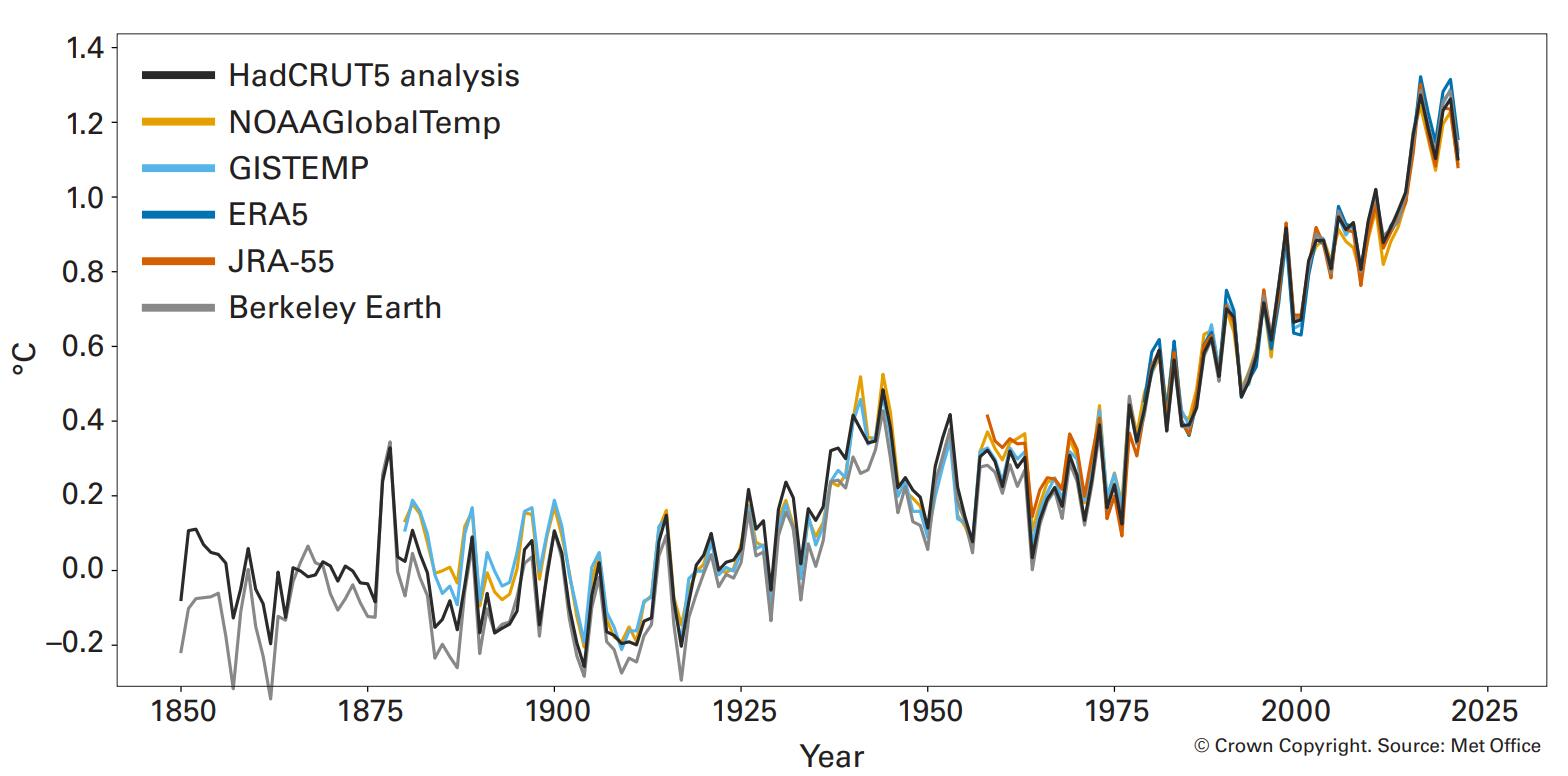
\includegraphics[width=13cm,height=3cm]{APMCMThesis/figures/six.jpg}
    \caption{Global annual
mean temperature
difference from
pre-industrial conditions
(1850–1900)\cite{bib:two}}
\label{fig1}
\end{figure}
Since the data in 2022\_APMCM\_C\_Data only cover up to September 2013, we collected the average temperature values  from six authoritative global temperature datasets up to October 2022. As the line graph\cite{fig1} shows, we could not agree more about global warming.



From NOAA\cite{bib:one} we extracted the average temperature for the last 10 years and visualized the data to show that the value for March 2022 is $+0.95^{\circ} \mathrm{C}\left(+1.71^{\circ} \mathrm{F}\right)$.
\begin{figure}
    \centering
    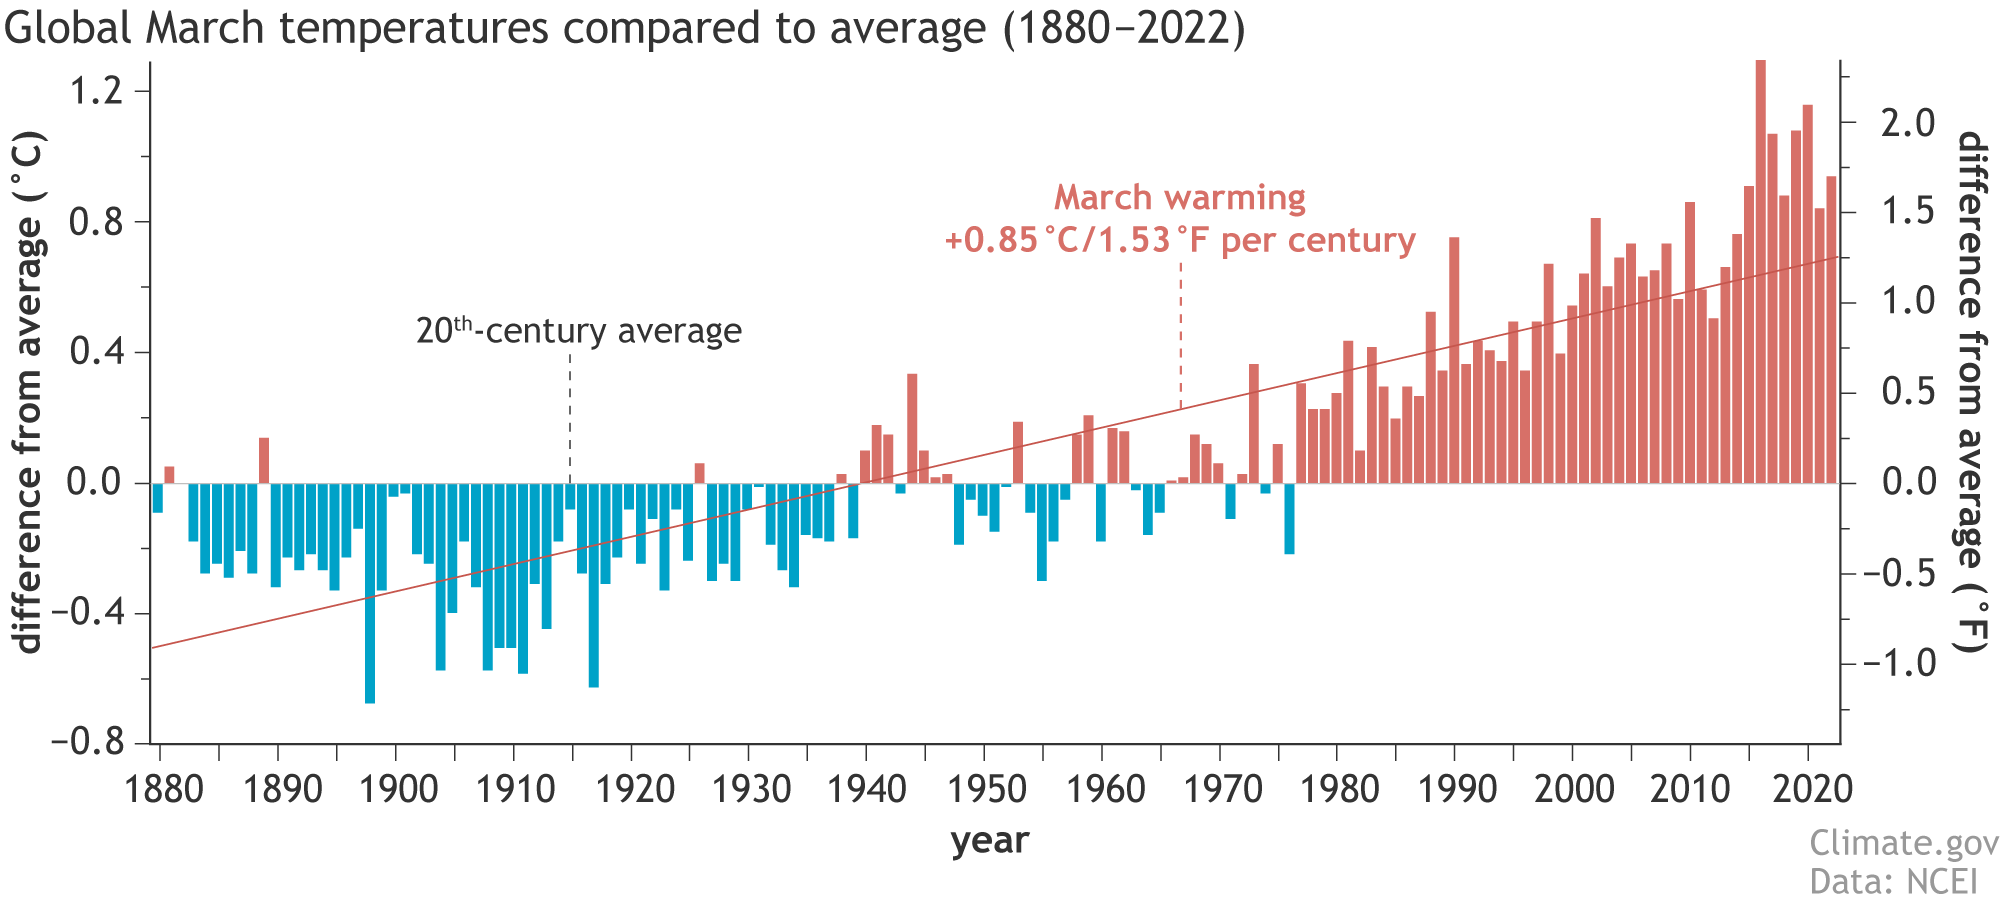
\includegraphics[width=13cm,height=5cm]{APMCMThesis/figures/Global_March2022_tempanom_graph.png}
    \caption{Global Land and Ocean Temperature Anomalies}
    \label{fig2}
\end{figure}

The March 2022 global surface temperature\cite{fig2} departure was the fifth highest for March in the 143-year record at 0.95°C (1.71°F) above the 20th century average. This was also the highest monthly temperature departure since November 2020. The seven warmest Marches have occurred since 2015, while the 10 warmest Marches have occurred since 2002. 

% \begin{table}
% \centering
% \caption{March Ranks and Records}
% \begin{tabular}{llllllll} 
% \toprule
% \multirow{2}{*}{March}          & 

% \multicolumn{2}{l}{Anomaly}                                   & \multicolumn{2}{l}{Rank}               & \multicolumn{3}{l}{Records}  \\
%                                 & °C                            & °F                            & \multicolumn{2}{l}{(out of 143 years)} & Year(s)    & °C    & °F      \\
% \midrule
% \multirow{2}{*}{Land}           & \multirow{2}{*}{+1.66 ± 0.11} & \multirow{2}{*}{+2.99 ± 0.20} & Warmest & 8th                          & 2016       & 2.5   & 4.5     \\
%                                 &                               &                               & Coolest & 136th                        & 1898       & -1.71 & -3.08   \\
% \multirow{2}{*}{Ocean}          & \multirow{2}{*}{+0.68 ± 0.14} & \multirow{2}{*}{+1.22 ± 0.25} & Warmest & 5th                          & 2016       & 0.86  & 1.55    \\
%                                 &                               &                               & Coolest & 139th                        & 1904, 1911 & -0.5  & -0.9    \\
% \multirow{2}{*}{Land and Ocean} & \multirow{2}{*}{+0.95 ± 0.15} & \multirow{2}{*}{+1.71 ± 0.27} & Warmest & 5th                          & 2016       & 1.31  & 2.36    \\
%                                 &                               &                               & Coolest & 139th                        & 1898       & -0.68 & -1.22   \\
% \bottomrule
% \end{tabular}
% \end{table}
\begin{figure}[!h]
    \centering
    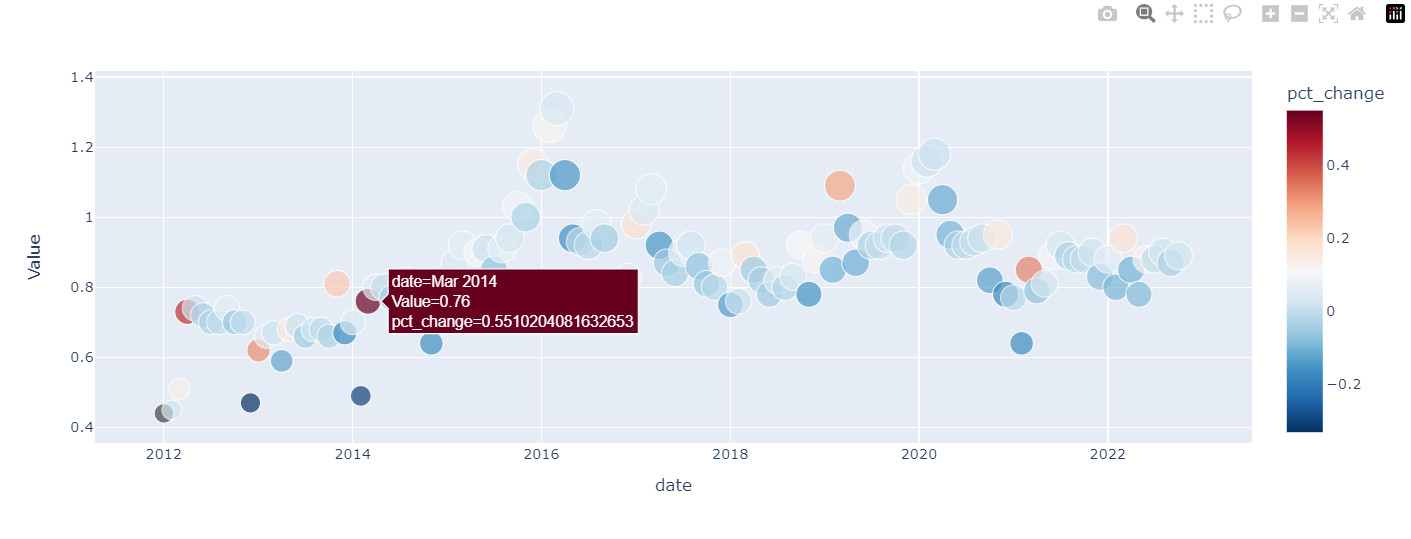
\includegraphics[width=15cm]{APMCMThesis/figures/增长率.png}
    \caption{Scatter plot of average temperature, where darker colors represent larger growth rates (2012-2022)}
    \label{fig3}
\end{figure}
By analyzing the data for this 10-year period, we learn that the maximum of these occurred in March 2016 and the largest year-over-year increase occurred in March 2014\cite{fig3}. In summary, the 22-year March temperature increase did not reach the largest increase in any previous 10-year period.

\subsection{Time Series Model}
In this section, we need to use historical temperature data to build a time series forecasting model.Time series forecasting is the task of fitting a model to historical, time-stamped data in order to predict future values. Traditional approaches include moving average, exponential smoothing, and ARIMA, though models as various as RNNs, Transformers, or XGBoost can also be applied. We built the model from both deep learning and statistical directions using the land mean temperature from 1750 to 2015 collected by Berkeley Earth.
\subsubsection{Temporal Fusion Transformer}
From a deep learning perspective, we used the Temporal Fusion Transformer (TFT) -- a novel attentionbased architecture which combines high-performance multi-horizon forecasting
with interpretable insights into temporal dynamics.

Let there be $I$ unique entities in a given time series dataset $-$ such as different citys in our temperature dataset. Each entity $i$ is associated with a set of static covariates $s_i \in \mathbb{R}^{m_s}$ like our Country,Latitude,Longitude, as well as inputs $\chi_{i, t} \in \mathbb{R}^{m_\chi}$ and scalar targets $y_{i, t} \in \mathbb{R}$ at each time-step $t \in\left[0, T_i\right]$. Time-dependent input features are subdivided into two categories $\boldsymbol{\chi}_{i, t}=\left[\boldsymbol{z}_{i, t}^T, \boldsymbol{x}_{i, t}^T\right]^T$ - observed inputs $\boldsymbol{z}_{i, t} \in \mathbb{R}^{\left(m_z\right)}$ which can only be measured at each step and are unknown beforehand, and known inputs $\boldsymbol{x}_{i, t} \in \mathbb{R}^{m_x}$ which can be predetermined (e.g. the day-of-week at time $t$ ).

In many scenarios, the provision for prediction intervals can be useful for optimizing decisions and risk management by yielding an indication of likely best and worst-case values that the target can take. As such, we adopt quantile regression to our multi-horizon forecasting setting (e.g. outputting the $10^{t h}$, $50^{t h}$ and $90^{t h}$ percentiles at each time step). Each quantile forecast takes the form:
$$
\hat{y}_i(q, t, \tau)=f_q\left(\tau, y_{i, t-k: t}, \boldsymbol{z}_{i, t-k: t}, \boldsymbol{x}_{i, t-k: t+\tau}, \boldsymbol{s}_i\right),
$$
where $\hat{y}_{i, t+\tau}(q, t, \tau)$ is the predicted $q^{t h}$ sample quantile of the $\tau$-step-ahead forecast at time $t$, and $f_q($.$) is a prediction model. In line with other direct$ methods, we simultaneously output forecasts for $\tau_{\max }$ time steps - i.e. $\tau \in$ $\left\{1, \ldots, \tau_{\max }\right\}$. We incorporate all past information within a finite look-back window $k$, using target and known inputs only up till and including the forecast start time $t$ (i.e. $y_{i, t-k: t}=\left\{y_{i, t-k}, \ldots, y_{i, t}\right\}$ ) and known inputs across the entire range (i.e. $\boldsymbol{x}_{i, t-k: t+\tau}=\left\{\boldsymbol{x}_{i, t-k}, \ldots, \boldsymbol{x}_{i, t}, \ldots, \boldsymbol{x}_{i, t+\tau}\right\}$ ).
\begin{figure}
    \centering
    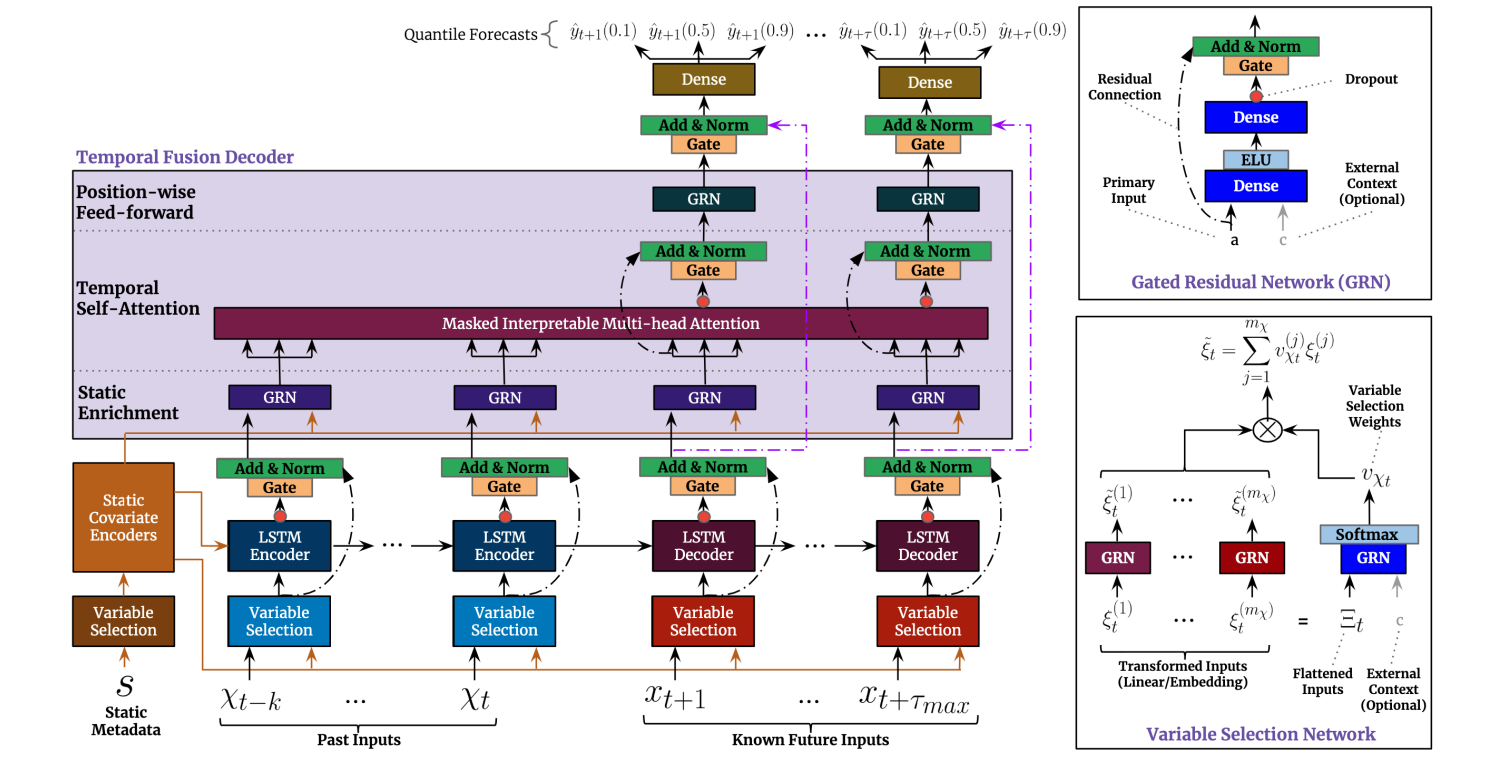
\includegraphics[width=13cm]{APMCMThesis/figures/TFT.png}
    \caption{TFT architecture\cite{2}}
    
\end{figure}

We design TFT to use canonical components to efficiently build feature
representations for each input type (i.e. static, known, observed inputs) for high
forecasting performance on a wide range of problems. The major constituents
of TFT are:
\begin{enumerate}
    \item \textbf{Gating mechanisms} to skip over any unused components of the architecture, providing adaptive depth and network complexity to accommodate a wide range of datasets and scenarios. 
    \item \textbf{Variable selection} networks to select relevant input variables at each time step.
    \item \textbf{Static covariate encoders} to integrate static features into the network,through encoding of context vectors to condition temporal dynamics.
    \item \textbf{Temporal processing} to learn both long- and short-term temporal relationships from both observed and known time-varying inputs. A sequenceto-sequence layer is employed for local processing, whereas long-term dependencies are captured using a novel interpretable multi-head attention block.
    \item \textbf{Prediction intervals }via quantile forecasts to determine the range of likely target values at each prediction horizon.
\end{enumerate}
\subsubsection{Prophet}
From a statistical point of view, we used Prophet\cite{3}.
Prophet is a procedure for forecasting time series data based on an additive model where non-linear trends are fit with yearly, weekly, and daily seasonality, plus holiday effects. It works best with time series that have strong seasonal effects and several seasons of historical data,and our average temperature data has exactly this characteristic. Prophet is robust to missing data and shifts in the trend, and typically handles outliers well.

Prophet is stated as a decomposable model with three main components: trend, seasonality, and holidays.

$$
y(t)=g(t)+s(t)+h(t)+\epsilon_t
$$

Where $g(t)$ is the trend function which models non-periodic changes in the value of thetime series, $s(t)$ represents periodic changes (e.g., weekly and yearly seasonality), $h(t)$ represents the effects of holidays which occur on potentially irregular schedules overone or more days. The error term $\epsilon_t$ represents any idiosyncratic changes which are not accommodated by the model.

This specification is similar to a generalized additive model (GAM) , a class of regression models with potentially non-linear smoothers applied to the
regressors. Here we use only time as a regressor but possibly several linear and non-linear
functions of time as components. Modeling seasonality as an additive component is the
same approach taken by exponential smoothing. Multiplicative seasonality,
where the seasonal effect is a factor that multiplies g(t), can be accomplished through a
log transform.

\subsection{Model Training}
In the Ubuntu conda environment we used autogluon, darts, and hyerts for training, and two RTX 3090 graphics cards for acceleration.

During the training process, we divide the average temperature of the last 10 years as the validation set, and plot the real value and the predicted value in a graph as a comparison.As you can see, there is barely any difference between the two.

\begin{figure}[!h]
    \centering
    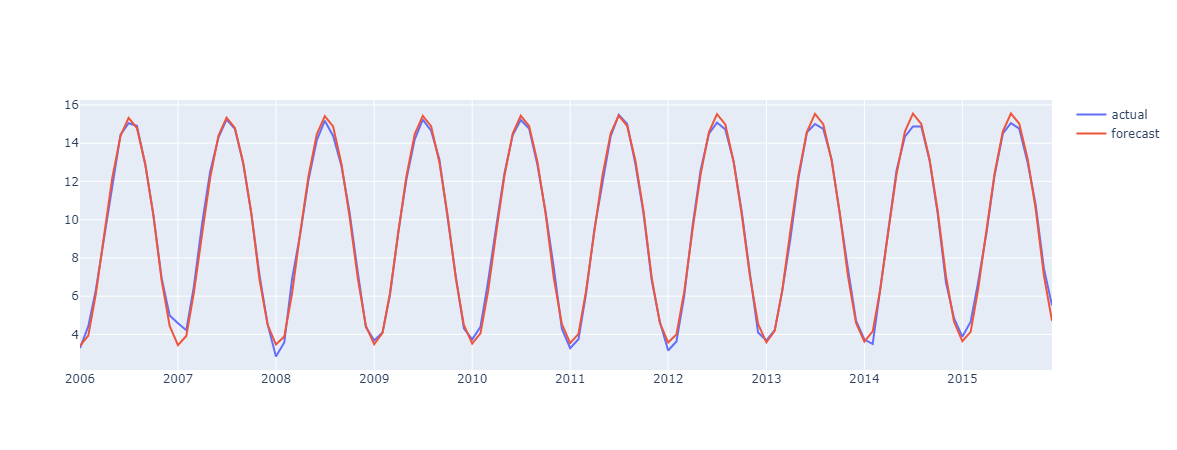
\includegraphics[width=13cm,height=3cm]{APMCMThesis/figures/0.png}
    \caption{Time-series prediction comparison chart}
    \label{fig:my_label}
\end{figure}

\subsection{Model Prediction}
We projected the monthly average temperature for the years 2016 to 2100 after training with 1000 epochs, making sure the model wasn't overfitted.

Using 20 degrees Celsius as the dividing line, the two models perform extremely differently, with Prophet projecting a stable and moderate global warming that won't reach 20 degrees until 2100, whereas TFT predicts a monthly global average land temperature of 20 degrees by June 2027.
\begin{figure}[!h]
    \centering
    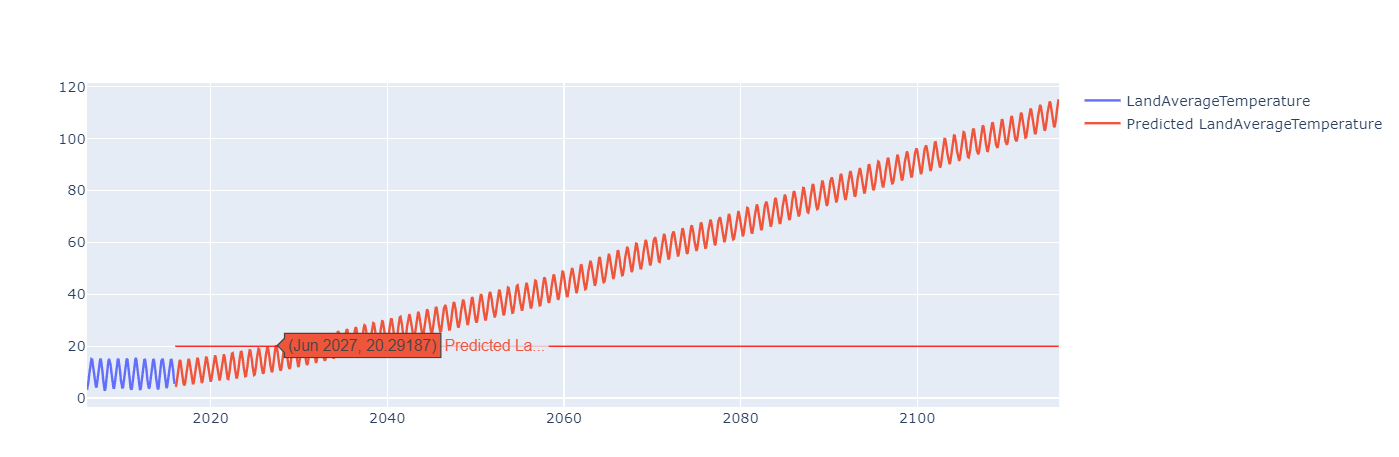
\includegraphics[width=13cm,height=3cm]{APMCMThesis/figures/pro.png} \\
    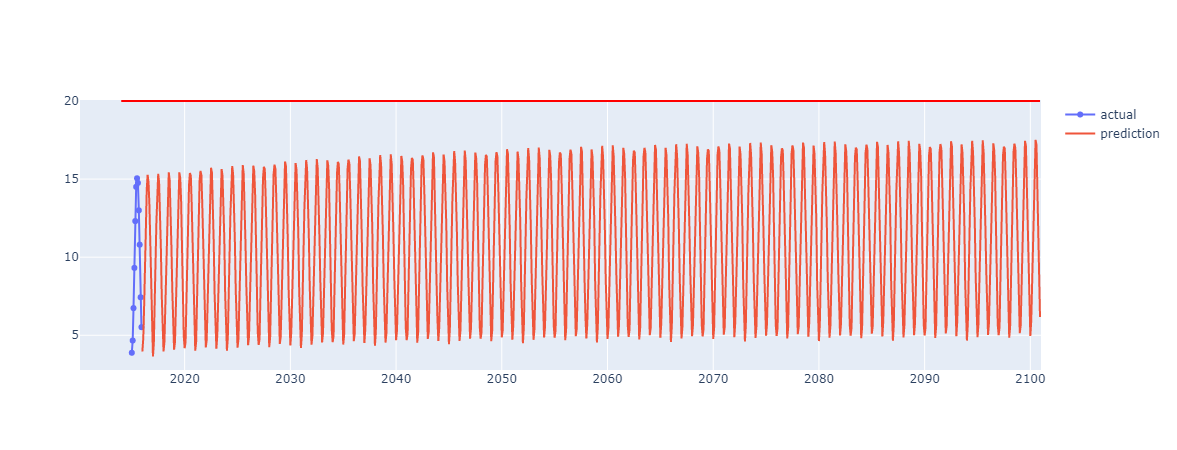
\includegraphics[width=13cm,height=3cm]{APMCMThesis/figures/model1.png}
    \caption{Predicted results (top: TFT, bottom: Prophet)}
    \label{fig:my_label}
\end{figure}

\subsection{Model Evaluation}
When the model's metrics are calculated to assess its performance, it is clear that TFT has a higher-performing model.
\begin{table}[!h]
\centering
\begin{tabular}{@{}lll@{}}
\toprule
Metirc & TFT    & Prophet \\ \midrule
mae    & 0.5032 & 0.6562 \\
mse    & 0.6200 & 0.9580 \\
smape  & 0.1114 & 0.9906   \\ \bottomrule
\end{tabular}
\caption{Performance Indicators}
\end{table}

In order to verify the conclusion that TFT is a better performing model, we back-tested the historical temperature data, plotted the temperature line graph for the past 15 years, and calculated the $R^2$ as 0.9905, so we believe that TFT is the more accurate model.
\begin{figure}
    \centering
    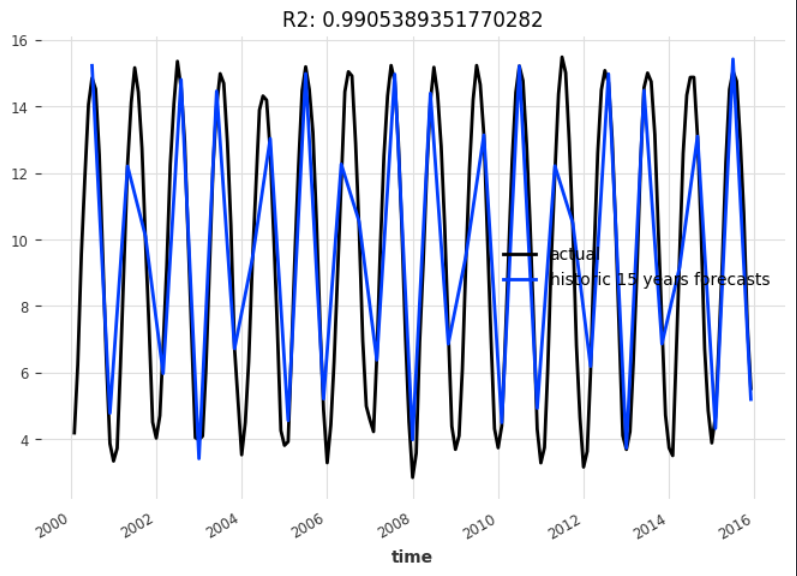
\includegraphics[width=10cm,height=3cm]{APMCMThesis/figures/R2.png}
    \caption{Backtest}
    \label{fig:my_label}
\end{figure}









\section{Model building and solution of question 2}
\subsection{Exploration of the relationship between temperature, time and location}
\subsubsection{Data Analysis \& Visualization}
First, using the dataset provided by APMCM, the monthly average temperature of a total of 100 cities can be analyzed and a heat map can be drawn on the world map\cite{hot}.
\begin{figure}[!h]
    \centering
    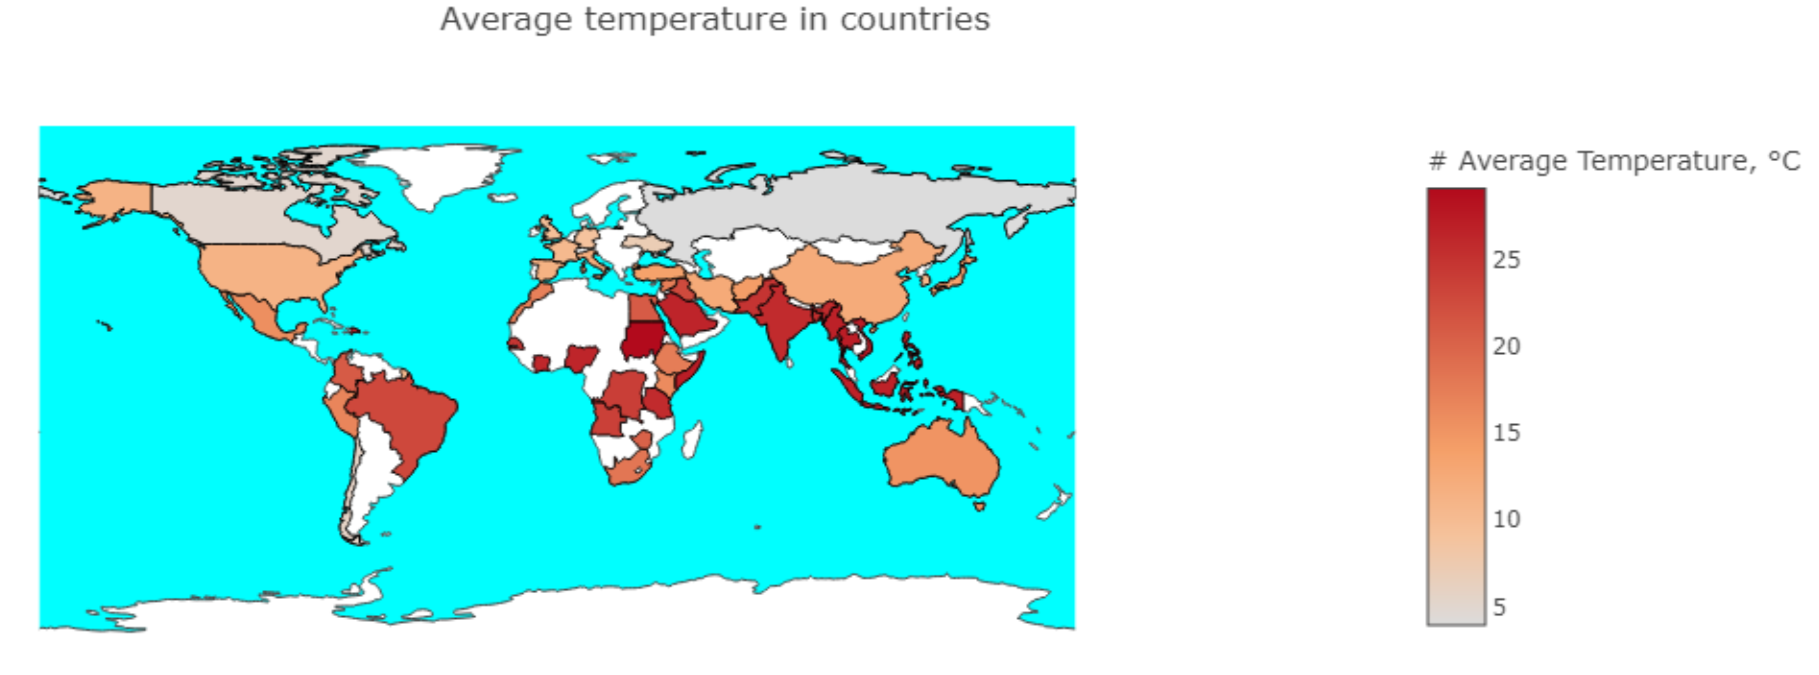
\includegraphics[width=13cm,height=3cm]{APMCMThesis/figures/hot.png}
    \caption{Global Temperature Map}
    \label{hot}
\end{figure}

It is not difficult to conclude from this that the average temperature of cities near the equator is higher, which is in line with objective common sense. However, it is not advisable to draw conclusions based on the naked eye alone. Next, we analyze the spatio-temporal relationship of temperature by model.
\subsubsection{Unraveled Multilevel Transformation Networks}
We use a deep learning model\cite{4} that learns to predict unknown
spatiotemporal dynamics using data from sparselydistributed data sites. We base our approach on Radial
Basis Function (RBF) collocation method which is
often used for meshfree solution of partial differential
equations (PDEs). The RBF framework allows us to
unravel the observed spatiotemporal function and
learn the spatial interactions among data sites on the
RBF-space. The learned spatial features are then used
to compose multilevel transformations of the raw
observations and predict its evolution in future time
steps. 

Consider our temperature sequence $\left(\mathcal{X}, \mathbf{u}_t\right), t=0,1, \cdots,(T+\tau-1)$ from a spatiotemporal dynamical system, where $\mathcal{X}=\left\{\mathbf{x}_1, \mathbf{x}_2, \cdots, \mathbf{x}_n\right\} \subset \Omega \subset \mathbb{R}^d$ being the set of data (measurement) sites and $\mathbf{u}_t=\left[u\left(t, \mathbf{x}_1\right), u\left(t, \mathbf{x}_2\right), \cdots, u\left(t, \mathbf{x}_n\right)\right]^{\top}$ being the corresponding data (measurement) values at time step $t$, with $u\left(t, \mathbf{x}_i\right) \in \mathbb{R}$. Given such $N$ examples $\left(\mathcal{X}^{(k)}, \mathbf{u}_t^{(k)}\right), t=0,1, \cdots,(T+\tau-1), k=1,2, \cdots, N$, find a (nonlinear) function $F: \mathbb{R}^{n \times d} \times \mathbb{R}^{n \times \tau} \rightarrow \mathbb{R}^{n \times T}, \tau>0, T>0$ that satisfies the conditions
$$
\mathbf{u}_{T+\tau-1}^{(k)}, \cdots, \mathbf{u}_{\tau+1}^{(k)}, \mathbf{u}_\tau^{(k)}=F\left(\mathcal{X}^{(k)}, \mathbf{u}_{\tau-1}^{(k)}, \cdots, \mathbf{u}_1^{(k)}, \mathbf{u}_0^{(k)}\right), \quad k=1,2, \cdots, N
$$

We consider representing the function $F$ as a deep neural network $F_\theta$, with parameter vector $\theta$. Here we propose an architecture for $F_\theta$ that is capable of modeling the spatiotemporal interactions of the underlying system. 
\begin{figure}
    \centering
    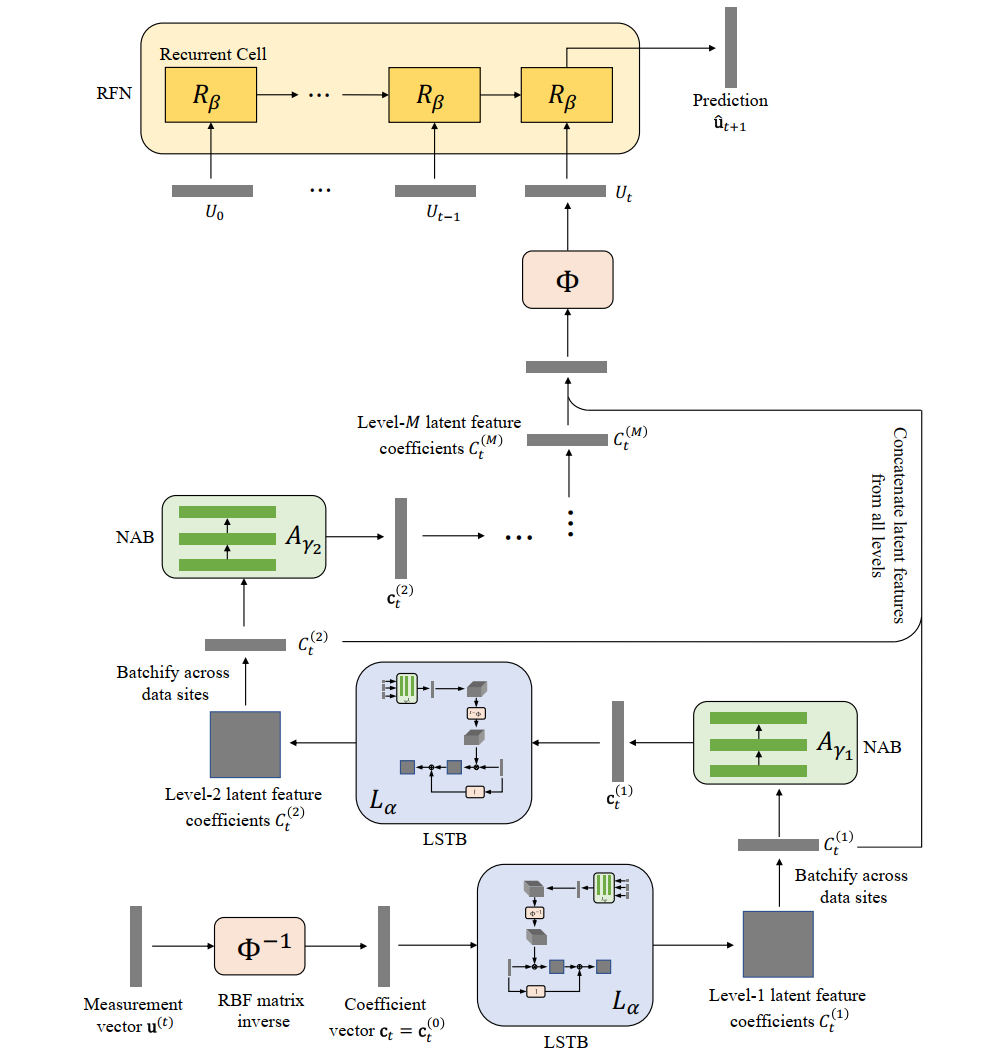
\includegraphics[width=13cm,height=8cm]{APMCMThesis/figures/umtn.png}
    \caption{End-to-end model involving multilevel transformations}
    \label{fig:my_label}
\end{figure}

The dataset we uesd contains saptiotempral sequences of SST generated by the NEMO ocean engine.The observations correspond to 250 randomly selected data sites within a $[0,550] \times[100,650]$ square cropped from the area between $50 \mathrm{~N}^{\circ}-65 \mathrm{~N}^{\circ}$ and $75 \mathrm{~W}^{\circ}-$ $10 \mathrm{~W}^{\circ}$ starting from 01-01-2016 to 12-31-2017. The data is divided into 24 sequences, each lasting 30 days (extra days in each month are truncated). Data corresponding to 2016 are used for training and the rest is used for validation and testing, in equal sequential split.
\begin{table}
\centering
\caption{March Ranks and Records}
\begin{tabular}{llll} 
\toprule
\multicolumn{2}{l}{Model~~ } & 15-step~~         & 25-step~~          \\
\midrule
     & 1-level~~             & 0:1526 ± 0:0009~~ & 0:1958 ± 0:0005~~  \\
UMTN & 2-level~~             & 0:1440 ± 0:0003~~ & 0:1820 ± 0:0003~~  \\
     & 3-level               & 0:1436 ± 0:0006~~ & 0:1812 ± 0:0009~~  \\
\bottomrule
\end{tabular}
\end{table}
\begin{figure}
    \centering
    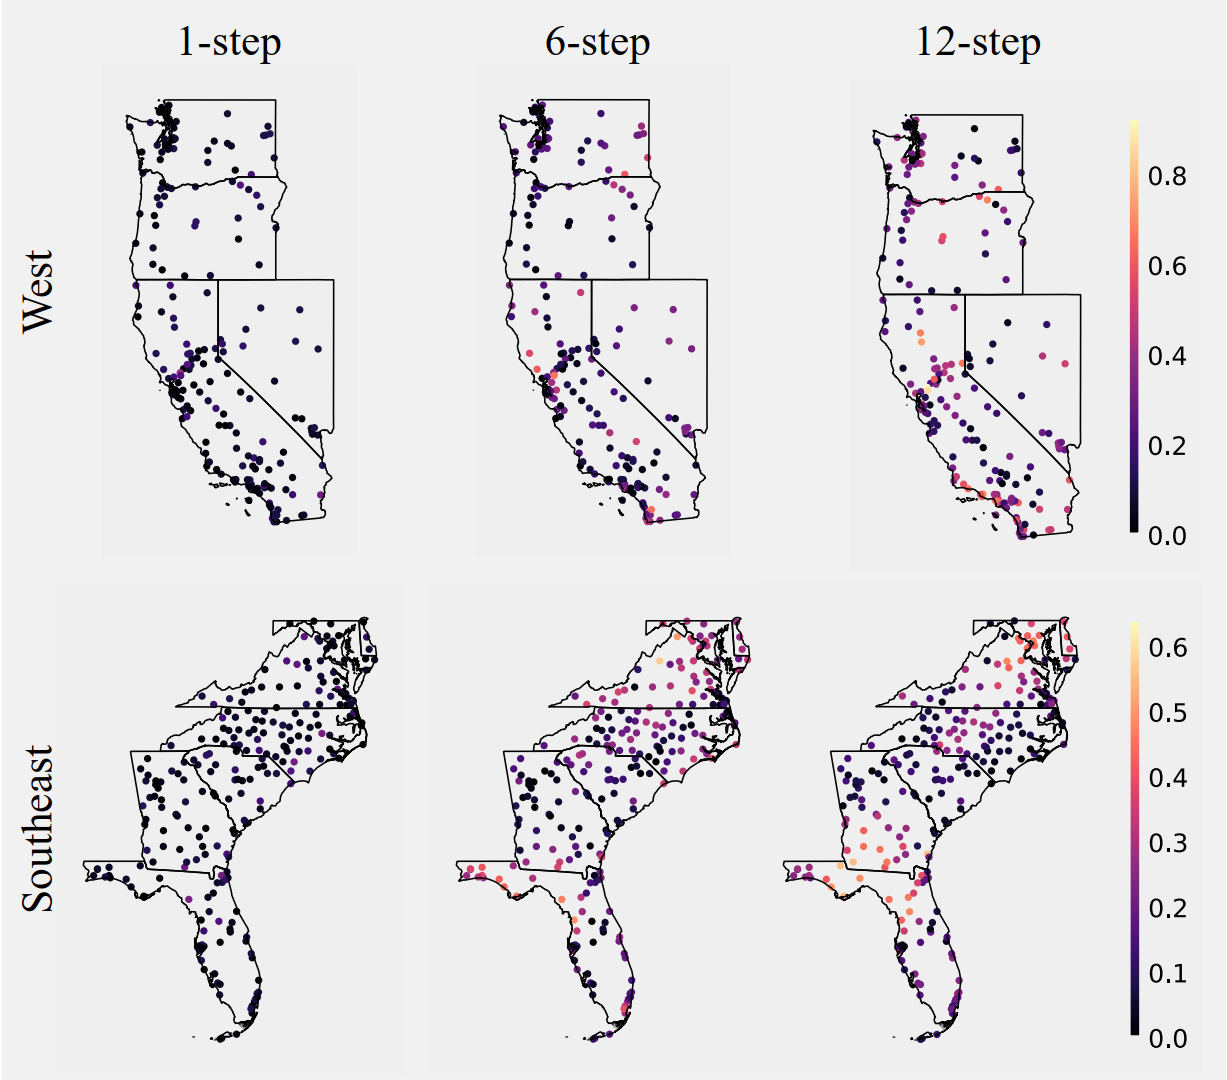
\includegraphics[height=6cm]{APMCMThesis/figures/mae.png}
    \caption{MAE distribution over time across data sites for our method in the NOAA experiment. All figures in each row
share the same colorbar, shown in the right of the corresponding row}
    \label{fig:my_label}
\end{figure}

We evaluate the methods on the tasks of predicting data (measurement) values at all the data sites for $T$ future time steps given observed values of the first $\tau$ time steps. We choose $\tau=5$ and investigate two cases: $T=15$ and $T=25$.

Table shows the prediction accuracy of different models in terms of mean absolute error. Our 3-level model outperforms the baselines in 25-step prediction. Drop in MAE from 1-level UMTN to 2-level UMTN is relatively larger than the drop in MAE from 2-level UMTN to 3-level and adding more levels contributes to negligible improvement in accuracy. 

We have introduced a framework for data-driven prediction of spatiotemporal dynamics when
data sites are sparse and irregularly distributed. The proposed method does not assume
any specific physical representation of the underlying dynamical system and is applicable to any spatiotemporal dynamical systems involving continuous state variables. We demonstrated
superior predictive performance of our model using both NOAA and SST temperature datasets. The
proposed method can be straightforwardly adapted to system involving multiple variables by
applying the LSTB to each of the measurement variables to create their corresponding linear
(spatial) differential features. NAB and RFN can then be used to learn the nonlinear relationships
among those linear (spatial) differential features of time,temperature and location.


\section{Natural factors affecting climate change}
In this question, we analyzed the impact of volcanic eruption and COVID-19 on global temperature. We collected data sets on the above two natural disasters and determined whether the above disasters would affect the global climate by establishing a correlation analysis model.

\subsection{Data preprocessing and visualization}
\subsubsection{COVID-19 dataset}
due to the unusual outbreak of COVID-19, almost every big and small cities 
and villages in the affected countries is under partial or total lockdown for a long period of time.

We collected data from NASA and European Space Agency (ESA) pollution monitoring satellites. The nitrogen dioxide ($NO_2$) over China is visualized as follows.\cite{no_2} We found that the areas of Eastern and Central China showed a significant reduction (10-30\%) in NO2 levels.

\begin{figure}
    \centering
    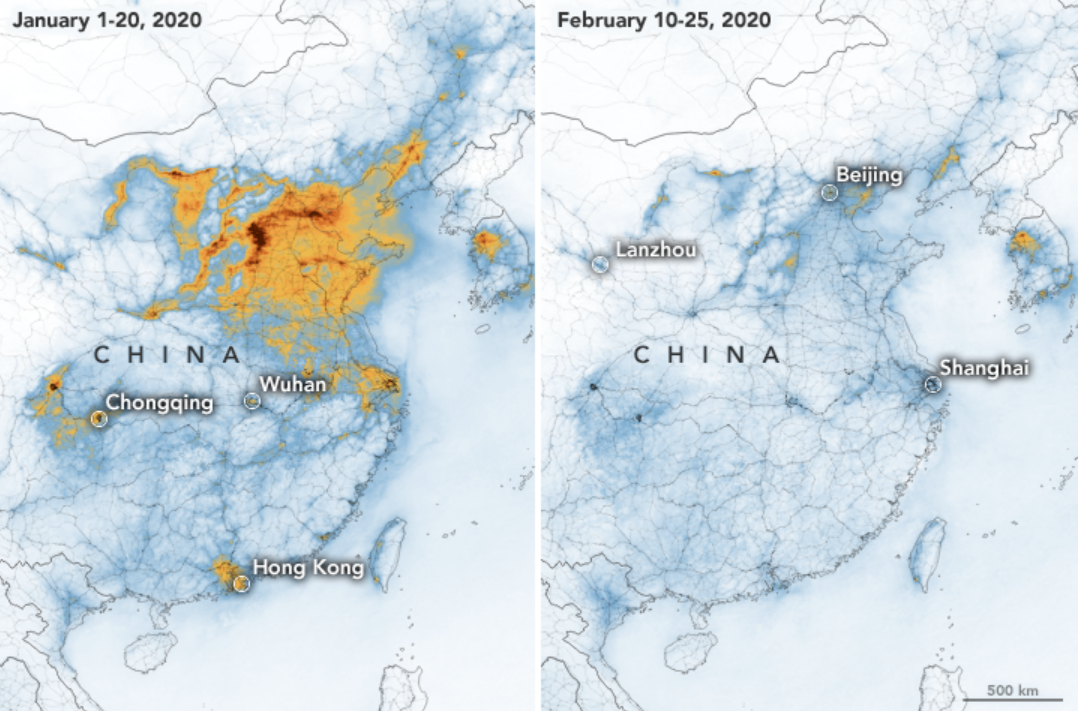
\includegraphics[width=9cm]{APMCMThesis/figures/china_no2.png}
    \caption{ $NO_2$ over China\cite{bib:two}}
\label{no_2}
\end{figure}     

 We have analysed 151 monitoring stations located across major Chinese cities in 31 provinces that track the concentrations of $\mathrm{PM}_{2.5}, \mathrm{PM}_{10}, \mathrm{O}_3, \mathrm{NO}_2, \mathrm{SO}_2, \mathrm{CO}$ in order to gather data before and after the outbreak of COVID-19. \cite{wuhan}.In addition, we collected air data of Wuhan and Beijing before and after the epidemic from Environmental and Energy Study Institute (EESI).In the cities of Wuhan and Beijing, our data indicsate a very diverse pattern in the concentration of pollutants after the outbreak of the disease. In Wuhan, all pollutants, except for ozone and sulphurdioxide, decreased substantially. Meanwhile, Beijing shows contractions only in $NO_2$ and $PM_10$, with the concentration of all other pollutants increasing over the time period under consideration. In Wuhan, the number of confirmed cases contributed to reducing the emissions of $PM_10$, $O_3$ and $NO_2$ by 6.55, 5.86 and 6.58 $μ/m^3$ respectively, while reducing PM2.5 by 17.9$ μ/m^3$ .


\begin{figure}
    \centering
    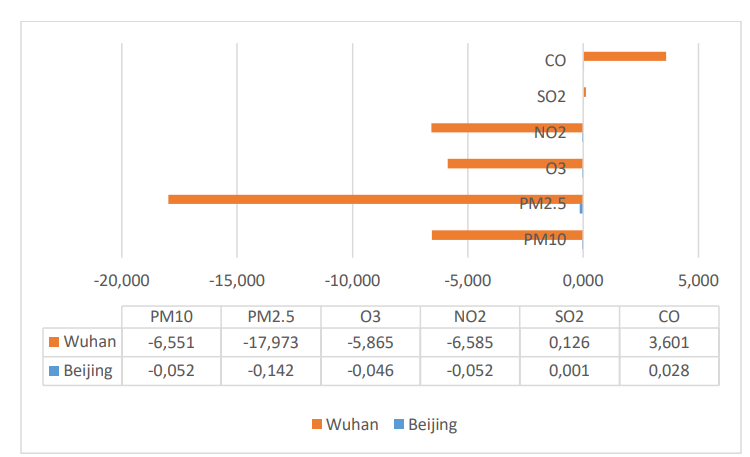
\includegraphics[width=9cm]{APMCMThesis/figures/wuhan.png}
    \caption{ The effects of the COVID-19 outbreak in Beijing and Wuhan\cite{bib:two}}
\label{wuhan}
\end{figure}    

 
In addition to Chinese data, we have collected data from NASA satellite sensors. 
We observed aerosol levels in northern India.\cite{india}
The first five maps above show aerosol optical depth (AOD) measurements over India during the same March 31 to April 5 period for each year from 2016 through 2020. The sixth map shows how AOD in 2020 compared to the average for 2016-2019.

\begin{figure}
    \centering
    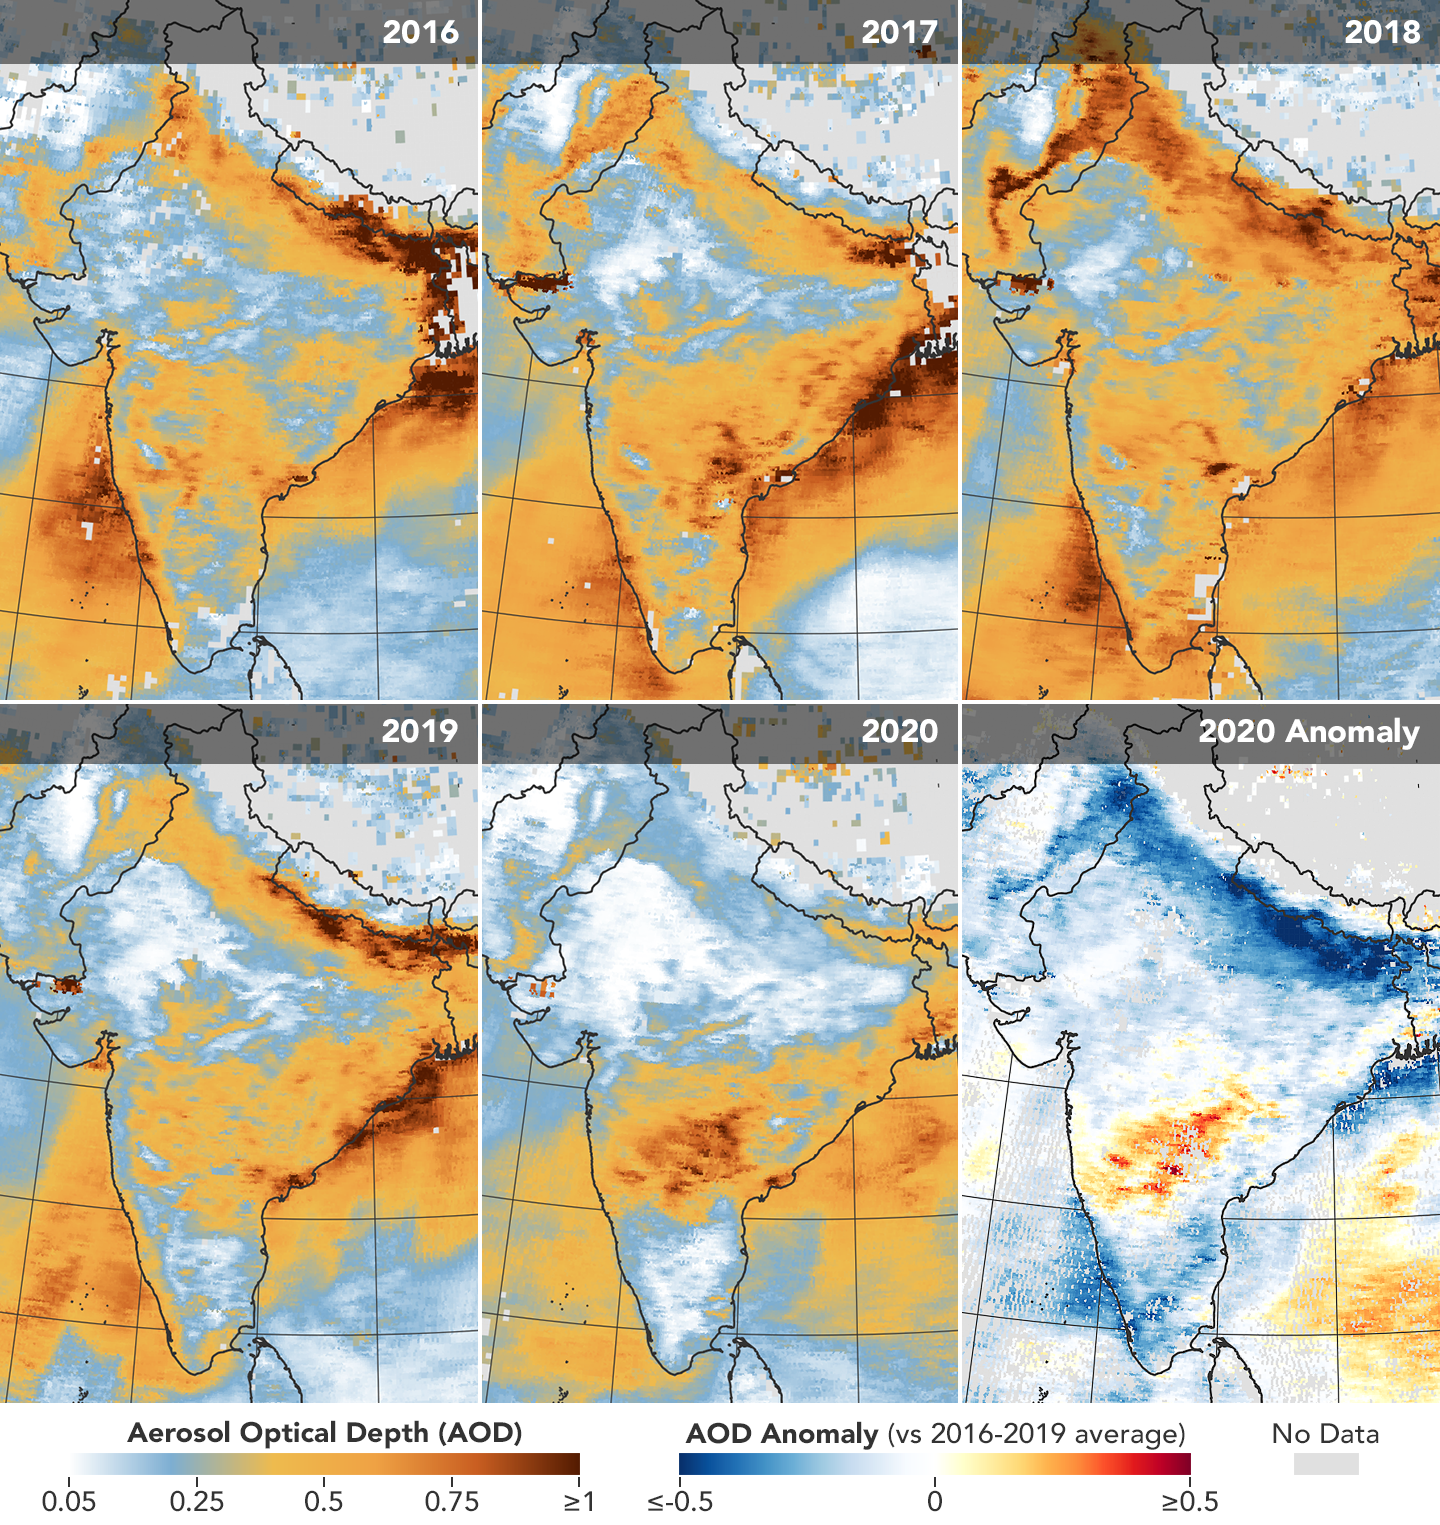
\includegraphics[width=13cm,height=5cm]{APMCMThesis/figures/india.png}
    \caption{ Airborne Particle Levels Plummet in Northern India\cite{bib:two}}
\label{india}
\end{figure}

\subsubsection{Volcanic eruption dataset}
We collected data on large-scale volcanic eruptions in the past 250 years.

 The global impact of large explosive and effusive eruptions, such as the 1991 eruption of Mount Pinatubo , the 1815 eruption of Tambora , or the 1783–1784 eruption of Laki, can be clearly seen in historical and environmental records . Injection of large quantities of volcanogenic material, such as fine tephra or volcanic gases (e.g. sulphur dioxide, carbon dioxide, hydrogen sulphide), into the stratosphere or troposphere can cause so-called `dust veil’ events \cite{21} with the potential to dramatically alter the Earth's climate on a regional or global scale for short periods of time (typically on the scale of several years to decades). The year following the 1815 eruption of Mt. Tambora, for example, is often referred to as the ‘Year Without a Summer’ – global temperatures are estimated to have dropped by 0.4–0.7 °C \cite{22}, causing several weather anomalies, particularly across the northern hemisphere.
 \begin{figure} 
    \centering
    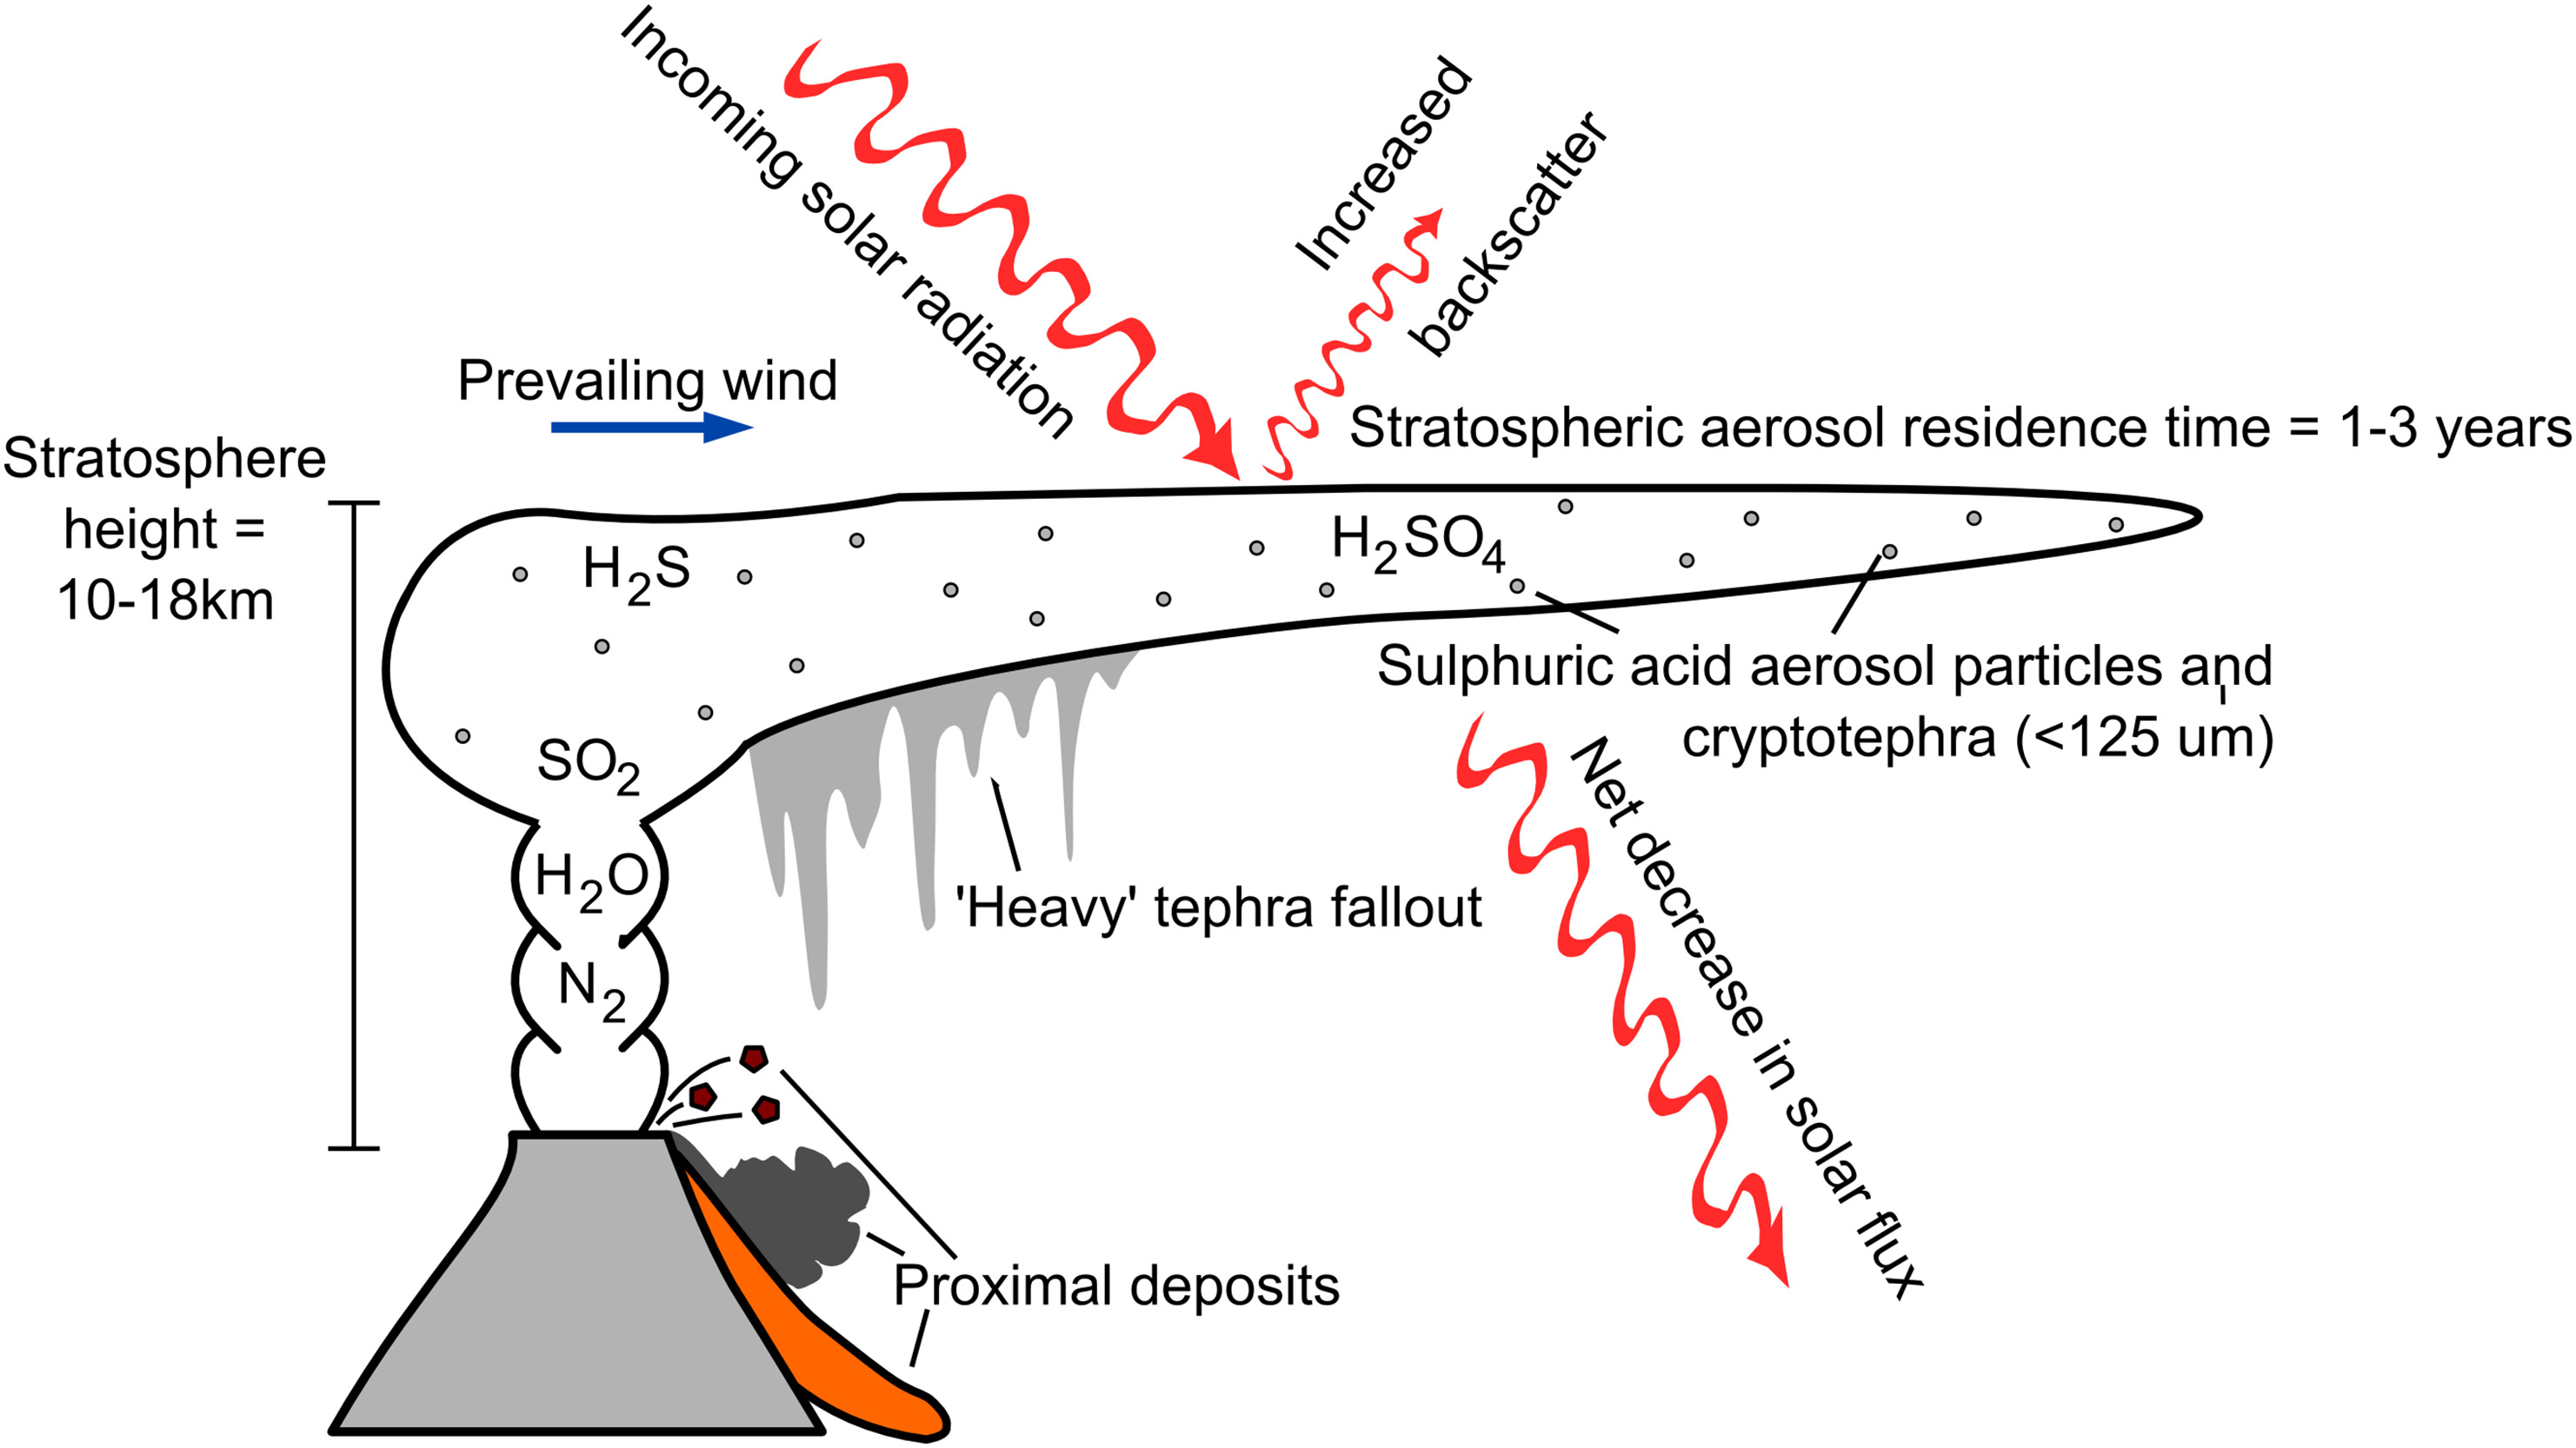
\includegraphics[width=10cm,height=3cm]{APMCMThesis/figures/volcanoe.png}
    \caption{Schematic of volcanic inputs to the atmosphere. Most tephra particles will fall out within a time period of days to weeks, while lighter emissions, such as gases and tephra particles < 125 μm in diameter may have a residence time of several months to years. Chemical species with a naturally high atmospheric abundance (such as $CO_2$, $H_2O$ and $N_2$) will have a much lesser effect than less common species, such as $SO_2$.}
\label{vol}
\end{figure}

\subsection{Model architecture}
The above data show the changes in greenhouse gases caused by the epidemic and volcanic eruptions. And we found that $CO_2$ concentration is much higher than other gases. Next, this paper will study the relationship between $CO_2$ concentration and average surface temperature from the perspective of energy balance. 

The average distance from the earth to the sun is about $1 \mathrm{AU}$ ,The radiation power of the sun on the outer layer of the earth perpendicular to the unit area of light is about $S=1370 \mathrm{~W} / \mathrm{m} 2$ .If the radius of the earth is $R$ ,the power radiated by the sun to the earth is, $S \cdot \pi R^2$ ,where  $\pi R^2$  is the effective area of the earth perpendicular to the light.However, about$30 \%$ of the solar radiation will be reflected back into space, that is, the albedo is abou $a=$ $0.3$ 。Considering the surface area of the earth is $4 \pi R^2$.Therefore, the solar radiation power obtained per unit area of the earth's surface is

$$
P_{\text {in }}=\frac{(1-a) \cdot S \cdot \pi R^2}{4 \pi R^2}=\frac{(1-a) S}{4}
$$

The energy output from the earth to outer space through long wave radiation can be calculated by treating the earth as a "black body". Stefan Boltzman law believes that the energy radiated from objects is proportional to the fourth power of their temperature. Therefore, the power output from the earth surface per unit area is

$$
P_{\text {out }}=\varepsilon \sigma T^4
$$

Where $\sigma=5.67 \times 10-8 \mathrm{~W} / \mathrm{m} 2 / \mathrm{K} 4$ is the Stefan Boltzmann constant. $\varepsilon$is the emissivity of the surface. For a perfect blackbody, $\varepsilon=1$ 。 $T$ is the earth surface temperature.The emissivity of ice is  $0.97$ ,and the emissivity of water is  $0.96$ , Water and ice are perfect black bodies. The difference between the input and output energy fluxes is called the radiative forcing and is expressed as

$$
\Delta F=P_{\text {in }}-P_{\text {out }}=\frac{(1-a) S}{4}-\varepsilon \sigma T^4
$$

If $\Delta F=0$ ,the temperature of the earth reaches equilibrium, and the equilibrium temperature of the earth is

$$
T_0=\left[\frac{(1-a) S}{4 \varepsilon \sigma}\right]^{1 / 4}
$$

If the greenhouse effect is not taken into account, the earth is close to the perfect black body. At this time,$\varepsilon=1$ 。Substitute $a=0.3 , S=1370 \mathrm{~W} / \mathrm{m} 2$ and $\sigma=$ $5.67 \times 10-8 \mathrm{~W} / \mathrm{m} 2 / \mathrm{K} 4$ into the above equation to get$T_0=255 \mathrm{~K}=-18{ }^{\circ} \mathrm{C}$  .In other words, if there is no greenhouse effect at all, the average surface temperature is about $-18{ }^{\circ} \mathrm{C}$ 。However, due to the normal greenhouse effect, the effective emissivity is less than 1$\varepsilon<1$ If the average surface temperature in 1951, 1980 is  $T_0=14.2^{\circ} \mathrm{C}=287.35 \mathrm{~K}$  the reference point (that is, it is considered that this temperature is the result of the normal greenhouse effect), according to which the effective emissivity of the earth can be calculated as $\varepsilon=0.6246$ 。

From the above analysis, it can be seen that human survival and development actually benefit from the greenhouse effect. If there is no greenhouse effect, the earth will be frozen.

However, due to the higher and higher concentration of greenhouse gases such as$\mathrm{CO} 2$in the atmosphere, the greenhouse effect is getting stronger and stronger. Greenhouse gases capture some of the energy that should be radiated into outer space, resulting in $\Delta F>0$. That is, the heat that the earth gets from the sun is greater than the heat that the earth radiates outward. In order to continue to maintain balance, the earth has to move from $T_ 0 $Raise the temperature $\Delta T$ to radiate more heat of $\Delta F$:

$$
\begin{aligned}
\Delta F &=\varepsilon \sigma\left(T_0+\Delta T\right)^4-\frac{(1-a) S}{4} \\
&=\varepsilon \sigma T_0^4\left(1+\frac{\Delta T}{T_0}\right)^4-\frac{(1-a) S}{4}
\end{aligned}
$$

Set $\varepsilon \sigma T_0^4=(1-a) S / 4$can be obtained by substituting the above equation
$$
\Delta F=\frac{(1-a) S}{4}\left[\left(1+\frac{\Delta T}{T_0}\right)^4-1\right]
$$

Considering  $\Delta T / T_0 \ll 1$ , $\left(1+\Delta T / T_0\right)^4$in the above equation can be expanded and approximated as
$$
\begin{aligned}
\left(1+\frac{\Delta T}{T_0}\right)^4 &=1+4\left(\frac{\Delta T}{T_0}\right)+6\left(\frac{\Delta T}{T_0}\right)^2+4\left(\frac{\Delta T}{T_0}\right)^3+\left(\frac{\Delta T}{T_0}\right)^4 \\
& \approx 1+4\left(\frac{\Delta T}{T_0}\right)
\end{aligned}
$$
so
$$
\Delta F \approx \frac{(1-a) S}{T_0} \Delta T \text { 或 } \Delta T \approx \frac{T_0}{(1-a) S} \Delta F
$$

In other words, there is an approximate linear relationship between the radiation  $\Delta F$ and the temperature increment$\Delta T$.
The study shows that $CO_2$ changes from the reference concentration . The radiative forcing caused by the increase of $C_0$ to $C$ can be calculated by the following formula:

:
$$
\Delta F_{\mathrm{CO}_2}=5.35 \ln \left(\frac{C}{C_0}\right)
$$

In the above equation,  $\mathrm{CO}$reference concentration $C_0$ represents reference temperature $T_0$ The   $\mathrm{CO} 2$ concentration corresponding to 0 is the average concentration of $\mathrm{CO}$ in the atmosphere from 1951 to 1980. Its value is about $320 \mathrm{ppm}$ . Considering that other greenhouse gases emitted by human activities should be positively correlated with the $\mathrm{CO}$emitted, this paper assumes that the total radiation intensity (including those caused by other greenhouse gases) is  $\Delta F$and the radiation forcing caused by  $\Delta F_{\mathrm{CO}_2}$ is proportional, i.e

$$
\Delta F=\eta \Delta F_{\mathrm{CO}_2}=5.35 \eta \ln \left(\frac{C}{C_0}\right)
$$

Where  $\eta$ is a constant. Substitute the above equation into the expression of temperature anomaly $\Delta T$ 
$$
\begin{aligned}
\Delta T & \approx \frac{5.35 \eta T_0}{(1-a) S} \ln \left(\frac{C}{C_0}\right) \\
&=\frac{5.35 \times 287.35 \eta}{(1-0.3) \times 1370} \ln \left(\frac{C}{C_0}\right) \\
&=1.603 \eta \ln \left(\frac{C}{C_0}\right)
\end{aligned}
$$

Where  $\eta$and  $C_0$are constants. The above equation gives the relationship between the surface average temperature anomaly $\Delta T$ and the $\mathrm{CO} 2$ concentration $C$ in the atmosphere. We can directly use this functional relationship to fit the$\mathrm{CO} 2$concentration and temperature profile anomaly. By fitting, $\eta=$ 2.3556、 $C_0=324.5$ , and the fitting curve is shown in\cite{co2}.

 \begin{figure} 
    \centering
    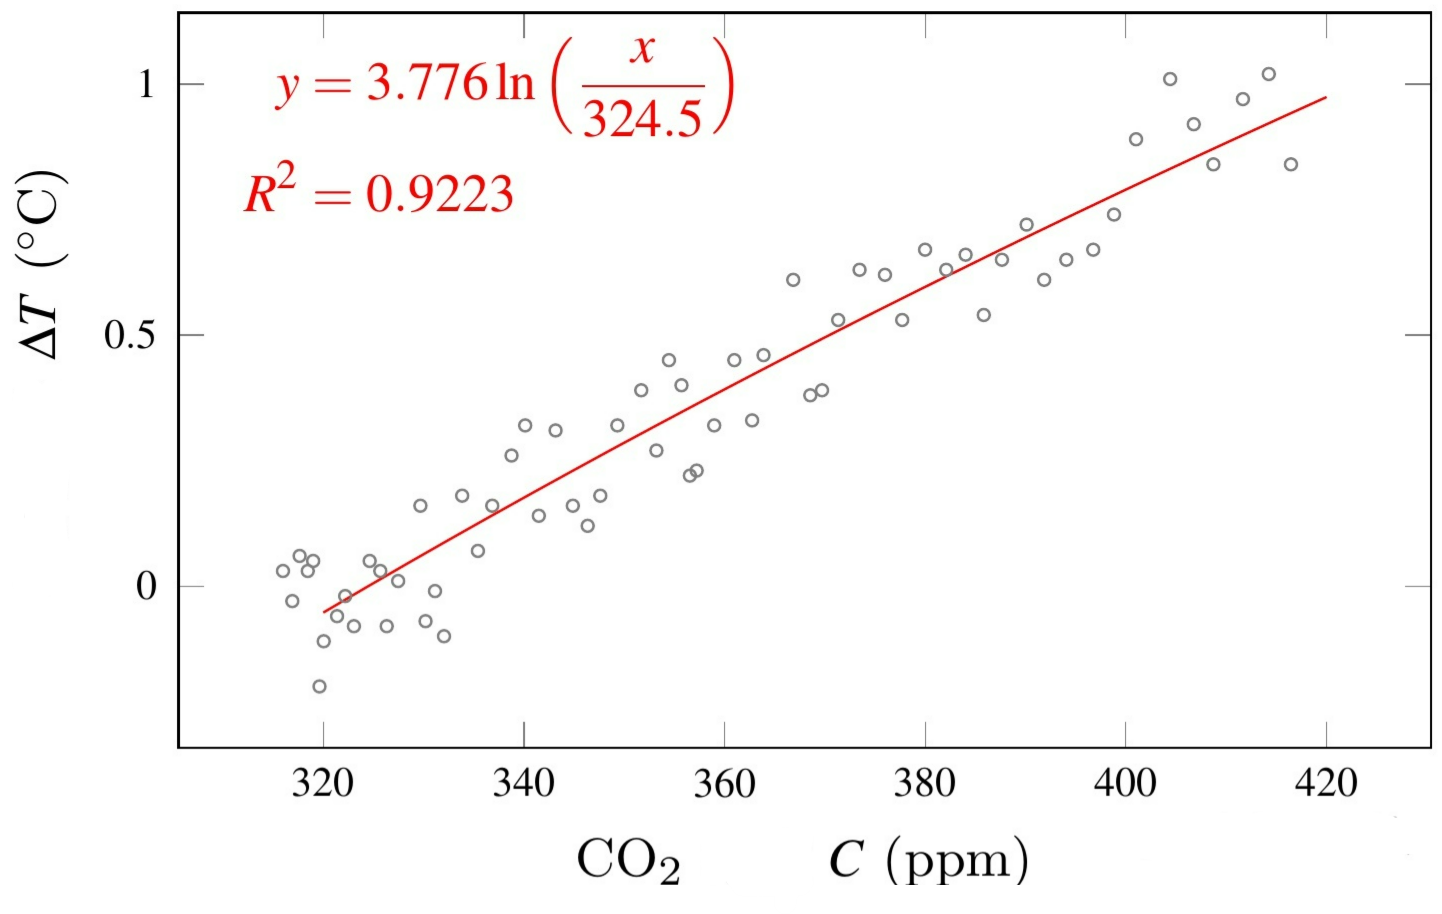
\includegraphics[width=9cm,height=3.5cm]{APMCMThesis/figures/co2.png}
    \caption{Fitting the relationship between carbon dioxide concentration and temperature}
\label{co2}
\end{figure}




\subsection{Results and analysis}
\subsubsection{Impact of COVID-19}
In the short term, COVID-19 has reduced human activities and gradually restored the ecology. But in the long run, the impact of COVID-19 on global temperature is negative.

During the COVID-19 epidemic, the environmental quality in many areas has significantly improved. However, the economic stagnation and mass unemployment make it difficult to celebrate the short-lived green. The International Energy Agency puts the reduction around 8 percent. That’s a meaningful reduction, and we would be in great shape if we could continue that rate of decrease every year. Unfortunately, we can’t.
But during the lockdown, emissions fell in the most expensive way, which is by halting the economy. After the pandemic, it would be difficult to oppose cheaper tools to achieve climate goals, such as carbon pricing. 

Perhaps the main reason why countries, firms and people have been so far reluctant in engaging in a serious and strong action to tackle climate change is due to its presumed high economic cost. The cost of halting the economy. Countries like Mexico, Spain or the UK have experience drops in GDP in double digits. The argument in favor of increasing carbon prices have in the past been depicted as an intolerable burden to society. 

 Let’s look at what it costs to avert a single ton of greenhouse gases\cite{cost}. If you have a technology that costs \$1 million, and using it lets you avert the release of 10,000 tons of gas, you’re paying \$100 per ton of carbon averted. 
If we treat the shutdown caused by COVID-19 as if it were a carbon-reduction strategy.In the United States, according to data from the Rhodium Group, it comes to between \$3,200 and \$5,400 per ton. In the European Union, it’s roughly the same amount. In other words, the shutdown is reducing emissions at a cost between 32 and 54 times the \$100 per ton that economists consider a reasonable price.
 
 Therefore, under the epidemic situation, many countries have been unable to pay for reducing carbon emissions due to economic recession.
 
  \begin{figure} 
    \centering
    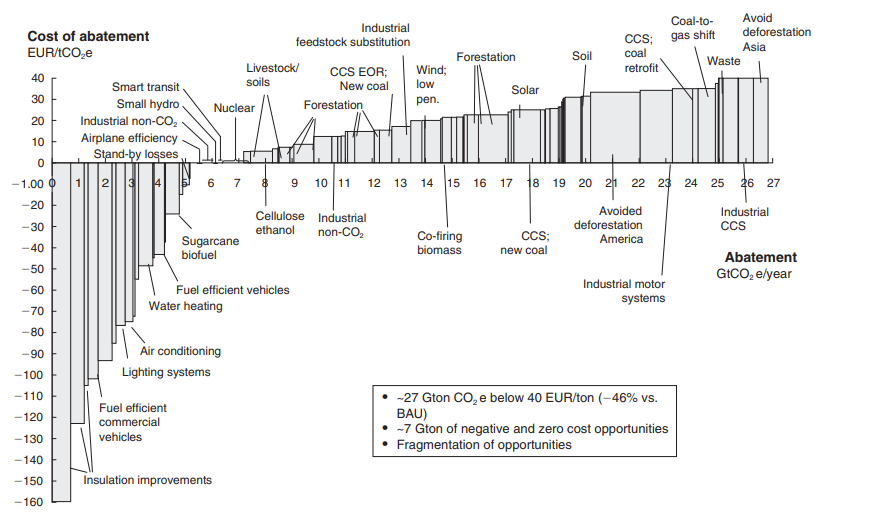
\includegraphics[width=9cm]{APMCMThesis/figures/cost.png}
    \caption{Ways to reduce the cost of carbon emissions}
\label{cost}
\end{figure}

 
\subsubsection{Impact of volcanic eruptions}
We analyzed the possible impact of volcanic eruptions.

Our data shows that the early eruption of the large igneous province will lead to a relatively short time of surface temperature reduction, sea level decline, and even the advent of the ice age; With the continuous eruption of magma, there will be a sudden long-term temperature rise, causing sea level rise, and even an ocean hypoxia event\cite{24}.These two different temperature effects are described below.

The contribution of volcanic gases such as sulphur compounds (e.g. $SO_2$, H2S) have a much greater impact on temperature.  If carried into the stratosphere by a volcanic column, these particles rapidly achieve global coverage, sometimes circulating the globe in as little as 3 weeks \cite{23}. The dominant effect of such an aerosol cloud is to greatly (albeit briefly) increase the planetary albedo by backscattering incoming solar radiation, resulting in net cooling at the surface.

But Stratospheric aerosol clouds produce winter warming over the continents in the NH. These and other effects are summarized in \cite{table_vol}. 
Individual large eruptions produce global or hemispheric cooling for 2 or 3 years, but the winter following a large tropical eruption is warmer over the NH continents.The winter warming pattern is illustrated in \cite{vol2}, which shows the global lower-tropospheric temperature anomaly pattern for the NH winter of 1991–1992 following the 1991 Mt Pinatubo eruption.

\begin{figure} 
    \centering
    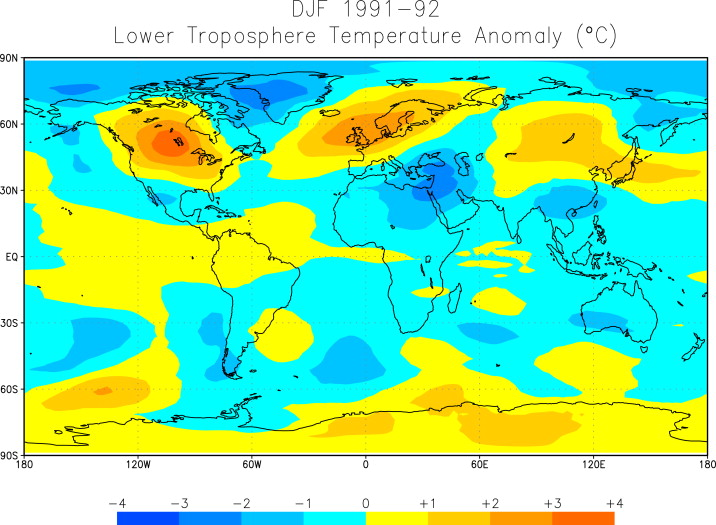
\includegraphics[width=9cm]{APMCMThesis/figures/vol2.png}
    \caption{Winter (DJF) lower-tropospheric temperature anomalies (with the nonvolcanic period of 1984–1990 used to calculate the mean) for the 1991–1992 Northern Hemisphere winter (DJF) following the 1991 Mt Pinatubo eruption. This pattern is typical of that following all large tropical eruptions, with warming over North America, Europe, and Siberia, and cooling over Alaska, Greenland, the Middle East, and China.\cite{bib:two}}
\label{vol2}
\end{figure}

The temperature over North America, Europe, and Siberia was much higher than normal and that over Alaska, Greenland, the Middle East, and China was lower than normal.


\begin{table}
\centering
\begin{tabular}{lll} 
\toprule
Effect/Mechanism                                 & Begins      & Duration         \\ 
\midrule
Stratospheric warming                            & 1-3 months  & 1-2 years        \\
Global cooling                                   & Immediately & 1-3 years        \\
Global cooling from multiple eruptions           & Immediately & Up to centuries  \\
Winter warming of Northern Hemisphere continents & 1 year      & 1 or 2 winters   \\
Reduced tropical precipitation                   & Immediately & 1 year           \\
Reduction of Asian and African summer monsoon    & 1 year      & 1 or 2 summers   \\
Ozone depletion, enhanced UV                     & 1 day       & 1-2 years        \\
\bottomrule
\label{table_vol}
\end{tabular}
\end{table}






\section{Main causes affecting global temperature change}
In addition to the above research contents, we also found some influencing factors that may lead to changes in global temperature, and they will dominate the global climate.
\subsection{Greenhouse effect}
During the accumulation process of greenhouse gases, the greenhouse effect is continuously accumulated. This accumulation will make the energy absorbed and released by the surface unable to reach a balance, and eventually the energy will accumulate and the temperature will rise, leading to global warming.

Greenhouse gases have always been the project indicators concerned by many scientists and human beings. They have high permeability to visible light from the sun, but can absorb infrared radiation from the surface. Such accumulation leads to the rise of the earth's temperature., However, since the middle of the 20th century, the content of all kinds of greenhouse gases in the atmosphere has increased with the advance of the industrial revolution and driven the global temperature rise.

The average mole fraction of global greenhouse gases was obtained from field observations at multiple sites planned by the Global Atmosphere Monitoring Program (GAW) of WMO and the partner network.\cite{101}

 \begin{figure} 
    \centering
    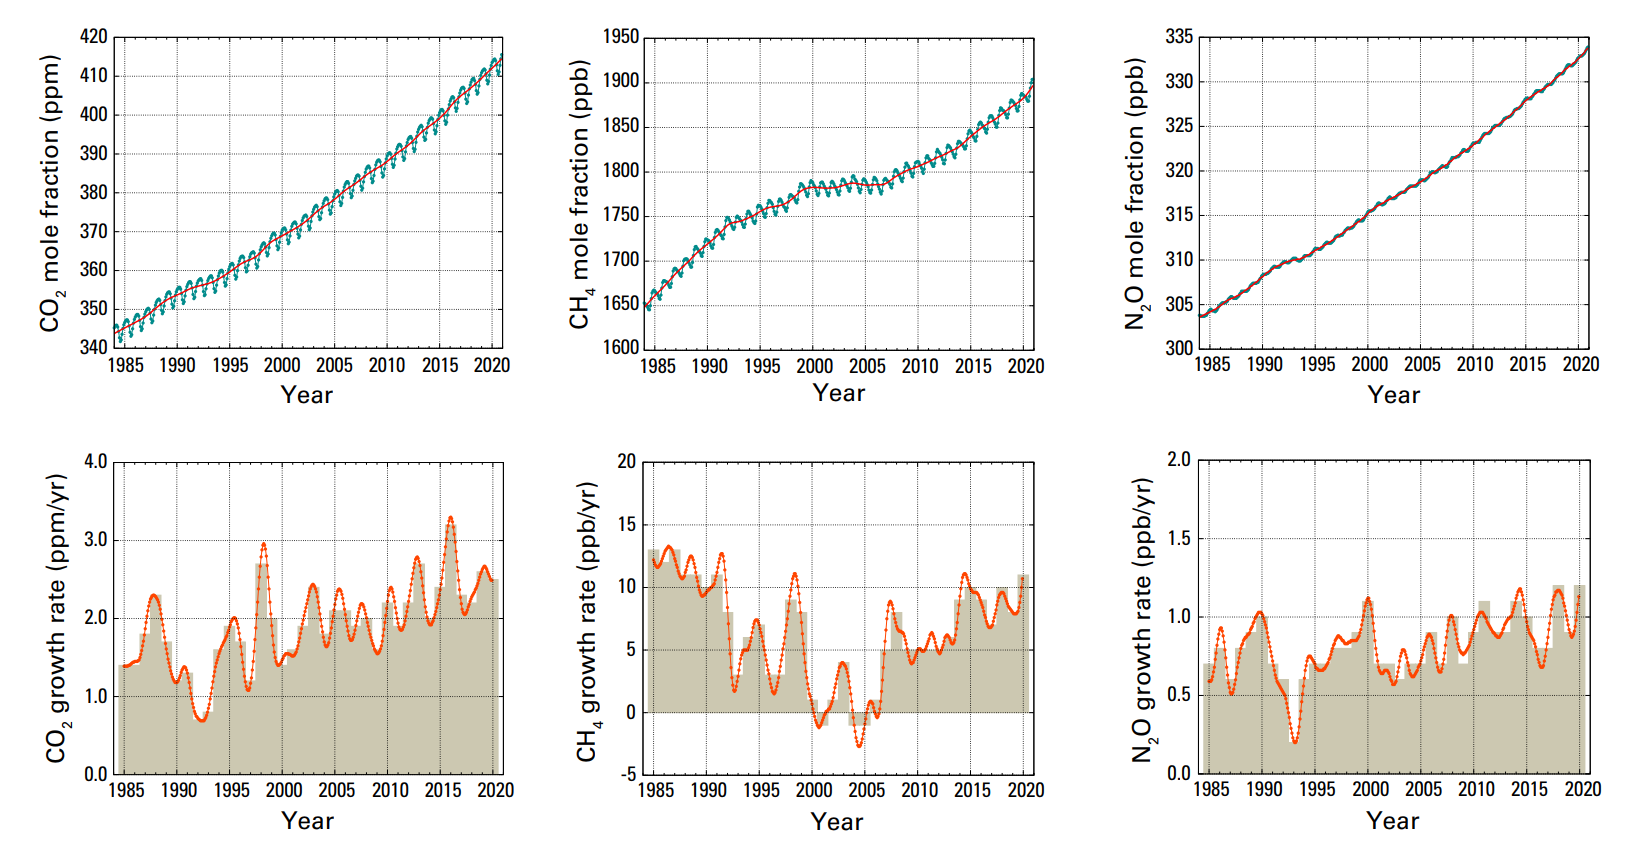
\includegraphics[width=14cm]{tu1.png}
    \caption{Molar fraction and growth rate of global greenhouse gases}
\label{growth}
\end{figure}

It can be seen from the observation data that the molar mass and growth rate of the three dominant greenhouse gases, $CO_2$, $CH_4$ and $N_2O$, in the air are gradually increasing. Although there was a short trough in the growth rate from 2000 to 2005, the ratio is still high, and according to the trend of the image, the molar mass of greenhouse gases will continue to increase gradually in the future, with no trend towards stability.

In 2020, the average mole fraction of global greenhouse gases will reach a record high. The carbon dioxide ($CO_2$) in this indicator will reach 413.2 ± 0.2 (ppm), 149$\%$ of the same indicator before industrialization. At the same time, $CH_4$ and $N_2O$ will also reach 262$\%$ and 123$\%$ of the same indicator before industrialization respectively. Due to the impact of COVID-19, global carbon emissions in 2020 will decrease by about 5.6$\%$ compared with 2019\cite{102}, but for $CH_4$ and $N_2O$, the growth rate in 2020 is still higher than that in the previous decade.

Therefore, in addition to the carbon dioxide emissions that people have always been concerned about, for example, the problem of $CH_4$ cannot be ignored. The increase of $CH_4$ content in the atmosphere has come into people's view, because it is also a powerful greenhouse gas that will cause serious damage to the ozone layer. The average growth rate of $CH_4$ kept a certain balance after the industrial revolution. It reached 12 ppb/year in the late 1980, and since then it has gradually declined, and almost dropped to zero between 1999 and 2006. However, since 2007, the growth rate has begun to rise again, and the growth rate in 2020 is about 11 ppb higher than that in 2019. The research shows that the emission of tropical wetlands and the emission of human activities in the mid latitudes of the Northern Hemisphere may be the leading reason for the increase of $CH_4$ content at present\cite{103}.

Take the greenhouse gas emission of the sewage treatment plant as an example. According to the statistics of developed countries, the carbon emission of the sewage treatment plant has accounted for 1.71$\%$ - 2.8$\%$ of the total\cite{104}. During the sewage treatment process, microorganisms are used to transform the organic matter in the sewage into inorganic matter through growth and reproduction, Various greenhouse gases are generated in this process, including:

\begin{itemize}
  \item $CO_2$ produced by microbial decomposition and respiration
  \item Methane bacteria participate in anaerobic fermentation of organic substances to produce $CH_4$
  \item $N_2O$, a by-product produced during nitrification and denitrification
\end{itemize}

According to the data reported by IPCC 2013\cite{105} on global warming potential, the calculated values of the three gases are $CO_2$: 1 (100 years), $CH_4$: 28 (100 years) and $N_2O$: 298 (100 years) respectively. Therefore, these three kinds of greenhouse gases generated in the sewage treatment process account for a very high proportion of the greenhouse effect generated by greenhouse gases.

Although in the IPCC 2006\cite{106}\cite{107} report, $CO_2$ was incorporated into the natural carbon cycle system for generation, and not separately included in the greenhouse gases generated by sewage discharge, in recent years, the detection technology of new science and technology found that the fossil carbon (FC) in the sewage plant is not $CO_2$ generated by biological metabolism, but has the same metabolic pathway, so it also contributes to the enhancement of the greenhouse effect.

$CH_4$ and $N_2O$ will have complex side reactions with other raw materials, gases in the air, devices, etc. in the complex treatment process. There are also many reactions whose mechanisms are not clear, but the reactions of greenhouse gas products can be detected.During the accounting, the different processes, uses and production methods will affect its emissions. According to the statistics of the United States, $N_2O$ generated by sewage treatment plants accounts for 3$\%$ of the national human emissions\cite{108}, ranking sixth in the global greenhouse gas emissions, which is also a big influencing factor.

To sum up, greenhouse gas emissions will be one of the most important factors in global warming. Most of the factories, farms and other places where people live or work will cause a lot of greenhouse gas emissions. When there is demand for production, we will inevitably cause biological or chemical factors to aggravate the greenhouse effect. Although such scenarios are difficult to eliminate, we can find ways to weaken them.

\subsection{Forest reduction}
Among the ways to reduce greenhouse gas emissions, the absorption of forests accounts for the vast majority. Because of the wide area of forests and their strong biological absorption of various greenhouse gases, their absorption capacity is superior to other artificial or unnatural absorption methods.

The reduction of forests is another major direction that affects global temperature change, not only because it can absorb a variety of greenhouse gases, but also because the existence of forests plays an important role in reducing natural disasters, maintaining biodiversity, and reducing desertification in oases. In recent years, natural disasters have occurred many times, desertification is serious, forest degradation, and it is difficult to maintain the ecological balance of the earth, The balance of gas content has led to the destruction of the ecosystem.

In 2005, the United Nations Framework Convention on Climate Change (COP11) proposed to reduce carbon emissions from deforestation in developing countries, and provided financial support. The proposal of the Convention attracted more people's attention to climate warming. However, the deforestation of tropical forests still has an impact on global climate change, and the ecosystem can store greenhouse gases underground, For example, the Amazon ecological community, in the early 1990s, the forest coverage has decreased by 11$\%$, about 700000 square kilometers, and the sharply reduced forest area is also greatly attacking its ability to mitigate the greenhouse effect.

The use of forests by people has led to the expansion of predatory production, which is gradually causing environmental degradation and will accelerate in 2020. The resurgence of deforestation can lead to cutting-edge progress in agriculture, but this method of opening up forest areas to increase agricultural production is not desirable. In addition, A large development area has been abused.

From 1990 to 2014, the proportion of Brazil's emissions in the world increased from 4$\%$ to 5$\%$, and its per capita emissions were far higher than the global average. In 2019, Brazil's emissions increased by 9.6$\%$. Due to deforestation, the emissions in Amazonia are nearly six times as large as those in the United States. Deforestation in Amazonia will promote the growth of carbon emissions in recent years. In particular, in deforestation, emissions from other sectors are also increasing gradually. As forests are cut down, the dynamic balance of biological communities is destroyed, and the carbon dioxide produced by these biological communities accounts for 87$\%$ of the sector.

As for Amazon, in 2005, this region accounted for 63.49$\%$ (1.2Gt $CO_2$) of the national MUT sector emissions (SEEG, 2019). Therefore, the renewable energy target in this region is estimated to be 719Mt $CO_2$ in 2025 and 887 Mt $CO_2$ in 2003.

According to the prediction of the deforestation scenario represented by the emission trajectory, through the collection of emission reduction data of Amazon forest from 2006 to 2020, a linear regression model is established to estimate the emission reduction data in 2025 and 2030.

 \begin{figure} 
    \centering
    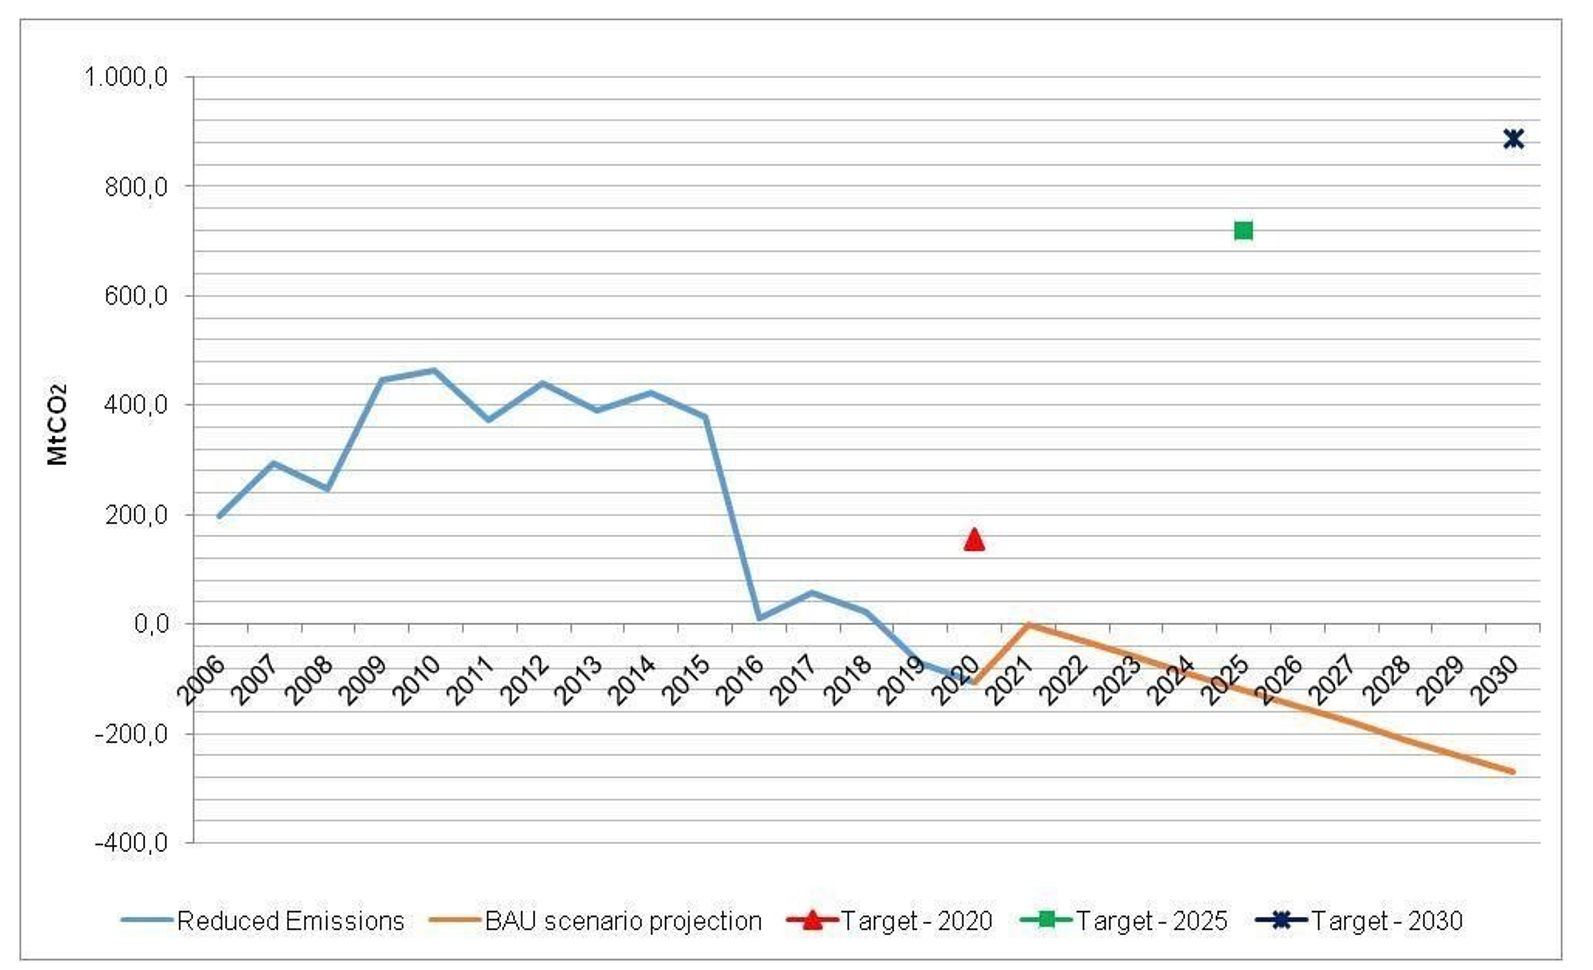
\includegraphics[width=13cm,height=3cm]{APMCMThesis/figures/tu2.png}
    \caption{Scenario Forecast of Emission Reduction and BAU in 2025 and 2030}
\label{recuction}
\end{figure}

According to the emission reduction data RE, a linear regression model is established, and the model results are as follows:

\text { REi }=-29.89+475.98 ti

 R² =  0.43, p values of α and β are 0.000 and 0.008, respectively. That is, since 2006, renewable energy has grown at an average rate of 475.98 million tons. By 2018, renewable energy has shown a growth trend.

% RE: Emission reduction
 % t: Year

However, it can be seen from the graph that since 2019, the ER estimates have shown a negative value, which means that the emission reduction has begun to show a negative trend, and the content of $CO_2$ in the atmosphere has begun to increase. The RE estimates in 2025 and 2030 are about -121.85 Mt $CO_2$ and -271.31 Mt $CO_2$, so the predicted values of the linear regression in 2025 and 2030 will show a negative value, that is, the emission reduction will still show a negative effect, which will conflict with the scheduled emission reduction goals.

This shows that the formulated emission reduction targets in the context of the Paris Agreement do not have a fully effective guiding significance. In recent years, the rate of forest loss is very high, which is far higher than the level of meeting environmental policies. Therefore, the reduction of emissions may be different from the expected value, which is also an important factor leading to current climate change. The emission reduction plans of various regions have a retrogressive or even reverse trend due to the reduction of forests, As a result, today's carbon emissions are still high.

\subsection{Human activities}
The current global warming is an artificial ecological reality. In the IPCC 2013 report, the Commission pointed out that "the study found that human activities have an impact on the rise of atmospheric and ocean temperature, the change of global hydrological cycle, the reduction of ice and snow, the rise of global average sea level and some extreme climate phenomena... The human impact is very likely the main reason for the warming observed since the middle of the 20th century"\cite{109}

Most of the factors we have studied that affect the global climate and temperature, such as the concentration of greenhouse gases, the generation of smoke and dust, and the thermal life activities of a large number of organisms, are inseparable from the impact of human activities, but also need human control. 

It can be reflected from the global average temperature level that the human impact on global warming can be attributed to two factors: human activity factors and the main participants in the change, so as to establish a tree chart.

 \begin{figure} 
    \centering
    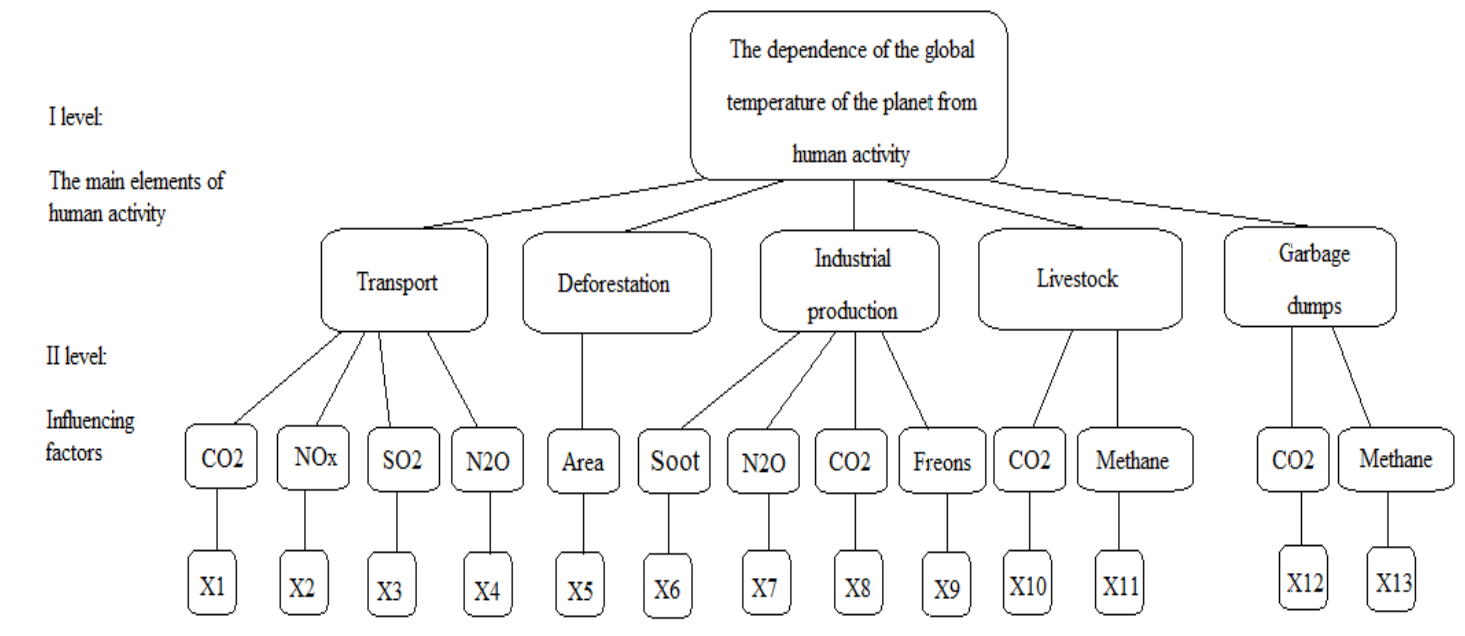
\includegraphics[width=13cm]{APMCMThesis/figures/tu3.png}
    \caption{Scenario Forecast of Emission Reduction and BAU in 2025 and 2030}
\label{relationship}
\end{figure}

It can be seen from the figure that the temperature rise caused by human activities can also be reflected in the following aspects in addition to what we have discussed:

\begin{itemize}
  \item Transportation. Vehicles used by human beings in modern times, led by cars, trains and airplanes, are the main contributors to global temperature rise. Due to the burning of fossil fuels, their carbon dioxide emissions have reached the forefront of various influencing factors. The transport sector is now the main contributor to energy consumption and greenhouse gas emissions. In 2015, the transport sector accounted for 24$\%$ of the global total carbon dioxide combustion emissions.
  \item Livestock breeding. In the process of livestock breeding, complex chemical or biological reactions occur in the accumulation, fermentation, and decomposition of excreta of feed, which is the main source of $CH_4$ in the atmosphere.  With the expansion of livestock breeding area, the potential impact of methane on the greenhouse effect will be more obvious.
  \item Garbage dump. The fermentation, decay and other complex reactions caused by the long-term accumulation of garbage lead to the continuous production of hydrogen sulfide, $CH_4$ and other harmful gases, which not only aggravate the greenhouse effect, but also cause poisoning due to the large amount of toxic gases accumulated.
\end{itemize}

Regardless of the impact of the general direction, personal impact alone, on November 15, 2022, the global population will reach 8 billion. Such a huge population base will make the carbon emissions and heat production of people in the world sharply increase. Due to different personal needs, from different aspects such as travel, technology, work, and even due to the heat production of people's own activities, this will still become a major factor affecting climate warming.

\section{Measures to curb or slow down global warming}
Many researches have been made on the impact of global warming, and various low-carbon agreements are common. Our traditional low-carbon ways include low-carbon travel, using environment-friendly energy materials, reducing electricity consumption, reducing the use of fossil energy, etc. However, according to the above official documents or data, such conventions may not play an effective role in prevention and control, The situation of increasing carbon emissions and global warming is still serious. Therefore, more and more emerging technologies have been put into research and development or use, hoping to deal with the peak of carbon emissions.

\subsection{New energy vehicles}
In view of the research on the emissions of traditional vehicles, it is found that the carbon emissions generated by burning fossil energy are huge. In contrast, the research found that the carbon emissions and heat release of new energy such as electric energy, solar energy, hydrogen energy are far less than those of traditional fossil fuel energy, and also contribute to carbon neutralization.

Take electric vehicles and electric buses as an example to count the emissions in energy production, and only consider the carbon dioxide emissions released in the process of energy consumption, and calculate the carbon emissions of traditional fuel vehicles \cite{111} at the same time, so as to make a clear comparison.

Electric vehicles do not consume carbon dioxide during production, transportation and driving. But if we consider the whole power cycle, according to the data provided by North China Power Grid (NCPG), the carbon emission coefficient is 1.246kg/kWh, but compared with the power effect, the emission is extremely small.

We measure the volume (L) of gasoline consumed by a car or bus every 100km, and according to the formula:

$$m_{c}=F_{g} \times V_{g}$$

%mc:$CO_2$ emissions per 100 km of vehicles/buses
%fg: $CO_2$ emission coefficient of gasoline
%vg:Volume of gasoline consumed per 100km

The $CO_2$ emissions of a fuel vehicle or bus for every 100km can be calculated.

\begin{table}
\centering

\begin{tabular}{ccll} 
\cline{1-2}
Types                                 & Electricity consumption \& $CO_2$~emission~~ &  &   \\ 
\cline{1-2}
$CO_2$ emission per 100km of one car     & 0 kg $CO_2$                                   &  &   \\ 

$CO_2$ emission per 100km of one person~~ & 0 kg $CO_2$                                   &  &   \\ 
\cline{1-2}
         & \multicolumn{1}{l}{}                      &  &  
\end{tabular}
\caption{$CO_2$ emission of electric cars}
\end{table}

\begin{table}
\centering
\begin{tabular}{ccll} 
\cline{1-2}
Total volume of gasoline per 100 km of one car & 10.49 L              &  &   \\ 
\cline{1-2}
$CO_2$ emission per 100km of one car              & 23.74kg $CO_2$           &  &   \\
$CO_2$ emission per 100km of one person~~         & 4.75kg $CO_2$            &  &   \\ 
\cline{1-2}
\multicolumn{1}{l}{}                           & \multicolumn{1}{l}{} &  &  
\end{tabular}
\caption{$CO_2$ emission of fuel cars}
\end{table}

\begin{table}
\centering
\begin{tabular}{ccll} 
\cline{1-2}
Types~~                                             & Electricity consumption  $CO_2$~emission 10.49 L &  &   \\ 
\cline{1-2}
Total electricity consumption per 100 km of one bus & 120kWh                                        &  &   \\
Carbon emission per 100km of one bus                & 0kg$CO_2$~~                                      &  &   \\
Carbon emission per 100km of one person~~           & 0kg$CO_2$~~                                      &  &   \\
\cline{1-2}
\end{tabular}
\caption{$CO_2$ emission of electric buses}
\end{table}

\begin{table}
\centering
\begin{tabular}{ccll} 
\cline{1-2}
Types~~                                & $CO_2$ emission~~       &  &   \\ 
\cline{1-2}
$CO_2$ emission per 100km of one bus      & 91.21kg $CO_2$          &  &   \\
$CO_2$ emission per 100km of one person~~ & 1.07kg $CO_2$~~         &  &   \\ 
\cline{1-2}
\multicolumn{1}{c}{~}                  & \multicolumn{1}{c}{} &  &  
\end{tabular}
\caption{$CO_2$ emission of fuel buses}
\end{table}

According to the data in the table, we can find that there is no carbon dioxide emission during the driving process of either electric vehicles or electric buses. Compared with traditional fuel vehicles, it reduces a lot of carbon dioxide emissions. We can think that electric vehicles have a strong contribution to reducing greenhouse gas emissions.

At the same time, we can also find that taking buses can also reduce carbon emissions per capita. According to statistics, the average annual total mileage of a private car in Beijing is 14332km\cite{112}, and the total carbon dioxide emissions are expected to reach 3.3 million tons. Therefore, the energy consumption and carbon emissions of electric vehicles are far lower than those of traditional cars. At the same time, buses can also reduce carbon emissions per capita, which will be strongly advocated in the future.

\subsection{Optimized Ridge – Furrow Ratio}
Agriculture is also a major source of greenhouse gases. In the process of crop growth, complex biological and chemical reactions will produce a variety of substances that cause global warming. With the development of the concept of sustainable development and the issuance of low-carbon goals, we hope that emerging technologies can reduce the greenhouse gas emissions that may be generated in the planting process to achieve the goal of low-carbon agriculture.

At present, plastic covered ridge and ditch rainwater collection system (RF) is widely used in the world, and RF coverage will affect soil conditions and the amount of greenhouse gases emitted. At present, research on the effect of ridge and ditch focuses on the use of covered materials, covering methods, etc. If an appropriate ridge and ditch ratio combination can be proposed, the greenhouse gases released by agriculture will be significantly reduced.

In the experiment, four random ridge and furrow treatments were used for wheat, respectively:

\begin{itemize}
  \item Uncovered (FP)
  \item RF40 (plastic covered ridge and ditch rainwater collection system, ridge and ditch ratio: 40:40cm)
  \item RF60 (ridge to ditch ratio: 40:60cm)
  \item RF80 (ridge to ditch ratio: 40:80cm)
\end{itemize}

\begin{figure} 
    \centering
    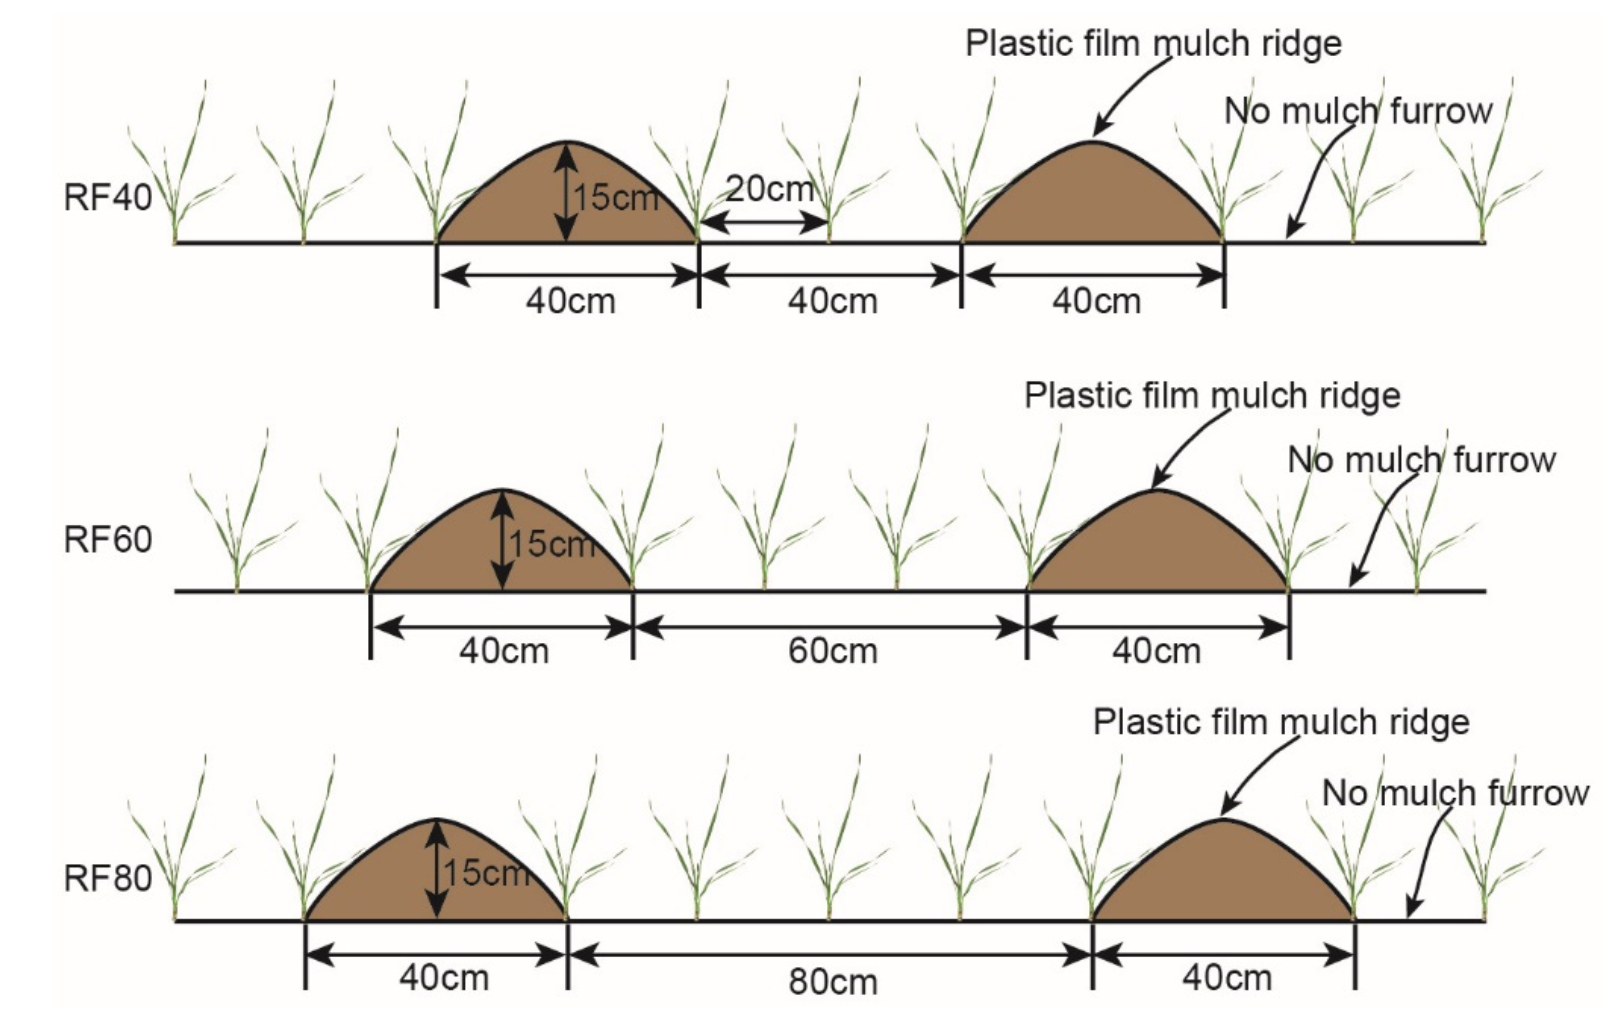
\includegraphics[width=11cm]{APMCMThesis/figures/tu4.png}
    \caption{Schematic Diagram of RF Experiment under Different Ridge Width}
\label{width}
\end{figure}

Use gas chromatograph, electron capture detector and flame ionization detector to analyze the concentration of $CO_2$, $CH_4$ and $N_2O$ in the gas sample within 42h, then the calculation method of gas emission flux is as follows:

$$F=\rho \times h \times \frac{d_{c}}{d_{t}} \times \frac{273}{T}$$

%F: the flux rate of $CO_2$, $N_2O$, and $CH_4$ ( )
%ρ: the standardized stage gas density of $CO_2$, $N_2O$, and $CH_4$ (mg cm−3) 
%h: the height of the chamber (m)
 %:the rate of greenhouse gas accumulation in the chamber
%T:the abAPMCMThesis/figures/tu5.pngute temperature




With the development of winter wheat, the $N_2O$ flux of each treatment decreased gradually and tended to be stable (A, B). The $N_2O$ flux increased from the first day, and reached the peak value around the seventh day under FP and RF respectively. During the growth period of this winter wheat, the $N_2O$ emission flux of RF was significantly higher than that of FP, and its cumulative emission flux was significantly increased by 419.84$\%$ than that of FP. In addition, the cumulative emission flux of RF80 was basically the same as that of RF40, but higher than that of RF60, and there was no significant difference among the three ridge to furrow ratios.

Based on the above research data, combined with the unified analysis of precipitation, soil temperature and humidity, it is found that in the years with more precipitation, the ridge to ditch ratio of 0:0 (i.e. conventional flat tillage) is applicable, while in the years with less precipitation, the ridge to ditch ratio of 40:71.3cm is applicable. At the same time, the greenhouse gas emissions can be achieved through the regulation of various ridge to ditch ratios. The above research results will best balance the greenhouse gas emissions and agricultural output, making sustainable agriculture more conducive to the mitigation of the greenhouse effect.




\newpage
%参考文献
\begin{thebibliography}{9}%宽度9
\bibitem{1} Rasmussen D J ,  Kulp S ,  Kopp R E , et al. Popular extreme sea level metrics can better communicate impacts[J]. Climatic Change, 2022, 170(3-4).

 \bibitem{bib:two} Kennedy J , Blunden J , J Alvar-Beltrán, et al. State of the Global Climate 2021. 2022.
\bibitem{bib:one} NOAA National Centers for Environmental information, Climate at a Glance: Global Time Series \url{https://www.ncei.noaa.gov/access/monitoring/climate-at-a-glance/global/time-series}
\bibitem{2} Lim B , Ark S , Loeff N , et al. Temporal Fusion Transformers for interpretable multi-horizon time series forecasting[J]. International Journal of Forecasting, 2021(1).
\bibitem{3} Taylor SJ, Letham B. 2017. Forecasting at scale. PeerJ Preprints 5:e3190v2
\bibitem{4} Saha P , Mukhopadhyay S . Unraveled Multilevel Transformation Networks for Predicting Sparsely-Observed Spatiotemporal Dynamics[J]. 2022.
\bibitem{20} R.A. Pielke, R. Avissar, M. Raupach, A.J. Dolman, X. Zeng, A.S. Denning Interactions between the atmosphere and terrestrial ecosystems: influence on weather and climate Glob. Chang. Biol., 4 (5) (1998), pp. 461-475
\bibitem{21}H.H. Lamb Volcanic dust in the atmosphere; with a chronology and assessment of its meteorological significance Philos. Trans. R. Soc. Lond. A, 266 (1178) (1970), pp. 425-533
\bibitem{22}R.B. Stothers The great Tambora eruption in 1815 and its aftermath Science, 224 (4654) (1984), pp. 1191-1198
\bibitem{23}A., M. Matson Circumglobal transport of the El Chichón volcanic dust cloud
Science, 224 (4654) (1984), pp. 1191-1198
\bibitem{24}郭正府,刘嘉麒.火山活动与气候变化研究进展[J].地球科学进展,2002,(04):595-604.



\bibitem{101} Kennedy J , Blunden J ,J Alvar-Beltrán, et al. State of the Global Climate 2020.  2021.
\bibitem{102}United in Science 2022: A multi-organization high-level compilation of the most recent science related to climate change, impacts and responses https://public.wmo.int/en/resources/united in science ; 
United In Science 2021: A multi-organization high-level compilation of the latest climate science information    https://library.wmo.int/index.php?lvl=notice display\&id=21946
\bibitem{103} Nisbet E G ,  Manning M R ,  Dlugokencky E J , et al. Very Strong Atmospheric Methane Growth in the 4Years 2014–2017: Implications for the Paris Agreement[J].  Global Biogeochemical Cycles, 2019, 33.
\bibitem{104}WANG H C. Carbon abatement in municipal wastewater treatment area
[J]. Water \& Wastewater Engineering, 2010, 36(12): 1-3, 52.

\bibitem{105}CHURCH J, CLARK P, CAZENAVE A, et al. Climate change 2013:
the physical science basis. An overview of the working group Ⅰ
contribution to the fifth assessment report of the intergovernmental
panel on climate change (IPCC) [J]. Geophysical Research Abstracts,
2014, DOI: 10.10161S0925-7721(01)00003-7.

\bibitem{106}LAW Y, JACOBSEN G E, SMITH A M, et al. Fossil organic carbon in wastewater and its fate in treatment plants[J].  Water Research, 2013,47(14): 5270-5281.
\bibitem{107} TSENG L Y, ROBINSON A K, ZHANG X Y, et al. Identification of preferential paths of fossil carbon within water resource recovery facilities via radiocarbon analysis[J]. Environmental Science \& Technology, 2016, 50(22): 12166-12178.
\bibitem{108}LAW Y, JACOBSEN G E, SMITH A M, et al. Fossil organic carbon in
wastewater and its fate in treatment plants[J]. Water Research, 2013,
47(14): 5270-5281.
\bibitem{109}D.F. Skripnuk, E.A. Samylovskaya, IOP Conf. Series: Earth and Environmental Science 180, 012021 (2018) doi :10.1088/1755-1315/180/1/012021
\bibitem{111}Zheng Z, Yang R, Yicheng H. The Energy Consumption and $CO_2$ emission impacts of Fuel and Electric Vehicles in China[C]//E3S Web of Conferences. EDP Sciences, 2021, 308: 01005.






\end{thebibliography}

% \newpage
% %附录

% \section{Appendix}
% \begin{lstlisting}[language=matlab,caption={The matlab Source code of Algorithm}]
% kk=2;[mdd,ndd]=size(dd);
% while ~isempty(V)
% [tmpd,j]=min(W(i,V));tmpj=V(j);
% for k=2:ndd
% [tmp1,jj]=min(dd(1,k)+W(dd(2,k),V));
% tmp2=V(jj);tt(k-1,:)=[tmp1,tmp2,jj];
% end
% tmp=[tmpd,tmpj,j;tt];[tmp3,tmp4]=min(tmp(:,1));
% if tmp3==tmpd, ss(1:2,kk)=[i;tmp(tmp4,2)];
% else,tmp5=find(ss(:,tmp4)~=0);tmp6=length(tmp5);
% if dd(2,tmp4)==ss(tmp6,tmp4)
% ss(1:tmp6+1,kk)=[ss(tmp5,tmp4);tmp(tmp4,2)];
% else, ss(1:3,kk)=[i;dd(2,tmp4);tmp(tmp4,2)];
% end;end
% dd=[dd,[tmp3;tmp(tmp4,2)]];V(tmp(tmp4,3))=[];
% [mdd,ndd]=size(dd);kk=kk+1;
% end; S=ss; D=dd(1,:);
%  \end{lstlisting}
% \begin{lstlisting}[language=c,caption={The lingo source code}]
% kk=2;
% [mdd,ndd]=size(dd);
% while ~isempty(V)
%     [tmpd,j]=min(W(i,V));tmpj=V(j);
% for k=2:ndd
%     [tmp1,jj]=min(dd(1,k)+W(dd(2,k),V));
%     tmp2=V(jj);tt(k-1,:)=[tmp1,tmp2,jj];
% end
%     tmp=[tmpd,tmpj,j;tt];[tmp3,tmp4]=min(tmp(:,1));
% if tmp3==tmpd, ss(1:2,kk)=[i;tmp(tmp4,2)];
% else,tmp5=find(ss(:,tmp4)~=0);tmp6=length(tmp5);
% if dd(2,tmp4)==ss(tmp6,tmp4)
%     ss(1:tmp6+1,kk)=[ss(tmp5,tmp4);tmp(tmp4,2)];
% else, ss(1:3,kk)=[i;dd(2,tmp4);tmp(tmp4,2)];
% end;
% end
%     dd=[dd,[tmp3;tmp(tmp4,2)]];V(tmp(tmp4,3))=[];
%     [mdd,ndd]=size(dd);
%     kk=kk+1;
% end;
% S=ss;
% D=dd(1,:);
%  \end{lstlisting}


\end{document} 